% =================================================================================
% Hier ausw�hlen, ob TUD-Design oder nicht
% =================================================================================
\newif\ifTUDdesign
\TUDdesigntrue					% TUD-Design
%\TUDdesignfalse				% F�r Rechner ohne installierte TUDdesign-Pakete
% =================================================================================


% =================================================================================
% Hier Daten f�r studentische Arbeit eingeben
% =================================================================================
\newcommand{\SADATyp}{Praktikumsbericht}
\newcommand{\SADATitel}{Praktikumsbericht\\}
\newcommand{\SADAStadt}{Stuttgart}
\newcommand{\SADAUnternehmen}{Vector Informatik GmbH}
\newcommand{\SADAAutor}{Samir Alexis Revelo Cordoba}
\newcommand{\SADABetreuer}{Dipl.-Ing. Hartmut H�rner}
\newcommand{\SADABetreuerII}{Dipl.-Ing. Markus Schwarz}
\newcommand{\SADABegin}{01. April 2016}
\newcommand{\SADAAbgabe}{31. September 2016}
\newcommand{\SADASeminar}{27. November 2013}


% =================================================================================


% =================================================================================
% Auswahl des IAT-Fachgebiets (rtm / rtp)
% =================================================================================
\newif\ifrtm
%\rtmtrue	% rtm
\rtmfalse	% rtp

% =================================================================================


% =================================================================================
% Erkl�rung, dass die Arbeit ohne Hilfe Dritter etc. erstellt wurde
% =================================================================================
\def\SADAVarianteErklaerung{ETIT}		% FB 18, Elektrotechnik
%\def\SADAVarianteErklaerung{MBDA}		% FB 16, Maschinenbau, Diplomarbeit
%\def\SADAVarianteErklaerung{MBSA}		% FB 16, Maschinenbau, Studienarbeit
% =================================================================================


% =================================================================================
% Ausnahmen von der automatischen Silbentrennung
% =================================================================================
\hyphenation{Aktu-ali-sie-rung Screen-shots Pa-rallel-ro-bo-ter Zu-stands-raum-mo-del-le nach-voll-zieh-bar Pro-jekt-se-mi-nar}
% =================================================================================


% =================================================================================
% Hier NIICHTS �ndern!
% =================================================================================
\ifTUDdesign
	\documentclass[11pt, twoside, colorback, accentcolor=tud9c, nopartpage, bigchapter, fleqn, ngerman, longdoc]{tudreport}
		
\else
	\documentclass[11pt, a4paper, twoside, fleqn, ngerman]{scrreprt}
  % F�r Entwurf auf Rechnern ohne installierte TUDdesign-Pakete	
	\usepackage{exscale}	% Korrektur math-Zeichen
	\usepackage{eurosym}
\fi
% Dieses File dient zum einbinden wichtiger und n�tzlicher Pakete.
% Nicht alle Pakete m�ssen verwendet werden.
%
\usepackage{t1enc}			% evtl. dc-Fonts
\usepackage[T1]{fontenc}	% F�r Silbentrennung bei W�rten mit Sonderzeichen (z.B. Umlaute)
\usepackage[latin1]{inputenc}
							% Um Sonderzeichen (�, �, �, ...) direkt eingeben zu k�nnen
\usepackage[english,ngerman]{babel}
							% F�r Sprachenspezifisches
							% ngerman ist schon als globale Option definiert

%\usepackage{helvet}			% Helvetica als Standard-Sans-Schriftart
\usepackage[stable]{footmisc}
\usepackage{booktabs}

\usepackage{sidecap}
\usepackage{graphicx}		% zum Einbinden von Postscript
\usepackage{psfrag}			% Beschriftung der Bilder
\usepackage{amsmath}		% Mehr mathematischen Formelsatz
%\usepackage{amssymb}		% Mehr mathematische Symbole
%\usepackage{amsthm}

\usepackage{float}			% F�r Parameter [H] bei Flie�objekten

\usepackage{epsfig}			% Um eps-Bilder einzubinden
\usepackage{scrhack}    % Um Warnung "float@addtolists detected" zu unterdr�cken 
\usepackage{subfig}			% F�r Unterabbildungen
\usepackage{ltxtable} 		% Vereinigt TabularX und Longtable
\usepackage{rotating}		% Zum Drehen von Objekten
\usepackage{bibgerm}		% F�r deutsche Literaturverwaltung
%\usepackage{wrapfig}		% F�r kleine Bilder am Rand
%\usepackage{floatflt}		% Alternative zu wrapfig
%\usepackage[hang]{caption}	% Damit mehrzeilige Bildunterschriften gut aussehen
\usepackage{upgreek}		% F�r nicht-kursive kleine griechischen Buchstaben

\usepackage{multirow}		% F�r mehrzeilige Felder in Tabellen

\usepackage{textcomp}		% F�r Sonderzeichen im normalen Text
							% (offensichtlich in tudreport schon eingebunden)
\usepackage[ngerman]{varioref}		% F�r vref
\usepackage{color}			% F�r farbigen Text
\usepackage{placeins}		% F�r \FloatBarrier
\usepackage{xspace}
\usepackage{icomma}			% Damit nach Dezimalkommas kein Abstand eingef�gt wird
							% (in math-Umgebungen)

\usepackage{cancel}			% Zum Wegstreichen von Gleichungstermen

\usepackage{array}			% F�r Zellentyp "m{}" in tabular-Umgebungen (Vertikal zentriert)

\usepackage{listings}		% Um formatierten Quellcode einzubinden
\usepackage{moreverb}		% F�r Umgebung "`verbatimtab"' (Verbatim mit Tabs)
\renewcommand{\verbatimtabsize}{4\relax}	% Standardtabweite in "`verbatimtab"'
											% ist 4 Zeichen


% Das Packet hyperref immer als letztes einbinden (nur bookmark darf danach kommen)!
%\usepackage[ps2pdf, colorlinks=false, pdfborder={0 0 0}]{hyperref}
%\usepackage[ps2pdf]{hyperref}	% F�r Verlinkungen im erzeugten pdf
\usepackage{hyperref}	% F�r Verlinkungen im erzeugten pdf
\usepackage{bookmark}

\usepackage{pdflscape} 
				% verwendete Pakete einbinden
% =================================================================================
% Definitionen f�r rtm / rtp
% =================================================================================
\ifrtm
	\newcommand{\SADAProf}{Prof. Dr.-Ing. Ulrich Konigorski}
  \newcommand{\SADAinstitut}{Institut f�r Automatisierungstechnik und Mechatronik\\
                             Fachgebiet Regelungstechnik und Mechatronik\\
                             \SADAProf}
  \newcommand{\SADAwebsite}{www.rtm.tu-darmstadt.de}
  \newcommand{\SADAtel}{06151/16-4167}
  \newcommand{\SADAlogo}{
\includegraphics[width=3cm]{./common/IAT_rtm}}
\else
  \newcommand{\SADAProf}{Prof. Dr.-Ing. Dr. h.c. Rolf Isermann}
  \newcommand{\SADAinstitut}{Institut f�r Automatisierungstechnik\\
                             und Mechatronik\\
                             FG Regelungstechnik und Prozessautomatisierung\\
                             \SADAProf}
  \newcommand{\SADAwebsite}{http://www.rtm.tu-darmstadt.de/rtp.html}
  \newcommand{\SADAtel}{06151/16-5465}
  \newcommand{\SADAlogo}{
\includegraphics[scale=0.5]{./rtp_fuer_tex/rtp_fuer_tex_RGB.pdf}}	
\fi

% =================================================================================		
% Definitionen Vector
	\newcommand{\SADAlogoVector}{
\includegraphics[scale=0.5]{./Bilder/vector-logo.pdf}}
	\newcommand{\SADAwebsiteVector}{https://vector.com/}
		
% =================================================================================
% Definitionen f�r die Erkl�rung, dass die Arbeit ohne Hilfe Dritter etc. erstellt wurde
% =================================================================================
% Die folgende Zeile deklariert die m�glichen Varianten der Erkl�rung, dass die
% Arbeit ohne Hilfe Dritter etc. erstellt wurde.
\def\ETIT{ETIT}\def\MBSA{MBSA}\def\MBDA{MBDA}
% =================================================================================


% =================================================================================
% Definitionen aus tudreport-Vorlage
% =================================================================================
\newif\ifTUDmargin
%\TUDmargintrue		% Sehr breiter rechter Rand
\TUDmarginfalse		% Schmaler (normaler) rechter Rand

\ifTUDmargin	% ggf. breiten Rand setzen
  \geometry{marginparsep=4.2mm,marginparwidth=28.64mm}
\fi

\newlength{\longtablewidth}
\setlength{\longtablewidth}{0.7\linewidth}
\addtolength{\longtablewidth}{-\marginparsep}
\addtolength{\longtablewidth}{-\marginparwidth}
% =================================================================================


% =================================================================================
% Farbige Deckseite, graue Balken auf allen anderen Seiten
% =================================================================================
\newif\ifOnlyColorFront
\OnlyColorFronttrue	    % Balken nur auf Deckblatt farbig
% \OnlyColorFrontfalse		% alle Balken farbig
% =================================================================================


% =================================================================================
% Befehle, die in scrreprt nicht exisiteren werden hier definiert, wenn diese
% Klasse verwendet wird.
% Auch die Seitenr�nder werden angepasst, so dass es grob wie mit tudreport
% aussieht.
% =================================================================================
\ifTUDdesign
	\title{\SADATitel}
	\subtitle{\SADAAutor}
	\subsubtitle{\SADATyp\ %-- \SADAAbgabe  
			\\Betreuer: \SADABetreuer{}, \SADABetreuerII{}
			\\Unternehmen: \SADAUnternehmen
			\\Abteilung: PES1}
	%\subsubsubtitle{\SADAUnternehmen}
	\setinstitutionlogo[height]{Bilder/vector_Logo_Typ_1}
	\geometry{left=30mm, right=20mm, top=15mm, bottom=20mm}
\else
	\title{\SADATitel}
	\subtitle{}
	\author{\SADAAutor}	% scrreprt erwartet Autor
	
	\newcommand{\subsubtitle}[1]{}
	\newcommand{\settitlepicture}[1]{}
	\newcommand{\printpicturesize}{}
	\newcommand{\institution}[1]{}
    \pagestyle{headings}

  % Diese Pakete nur extra einbinden, wenn NICHT tudreport als Basis.
	\usepackage{amssymb}
	\usepackage{geometry}
	
% \settitlepicture{}	% Bild f�r Deckblatt
% \printpicturesize
\fi
% =================================================================================


% =================================================================================
% Anpassung Absatzformat
% =================================================================================
% Der Abstand der Zeilen betr�gt das 1,25-fache des Standard-Abstands von
% LaTeX. Da technische Arbeiten viele Formeln und Bilder enthalten, werden
% Abs�tze durch einen zus�tzlichen vertikalen Zwischenraum statt durch einen
% Einzug getrennt.
\linespread{1.25}
\setlength{\parindent}{0mm}
\setlength{\parskip}{1ex}
% =================================================================================


% =================================================================================
% Texte f�r die R�ckseite des Titelblatts vorgeben
% =================================================================================
\uppertitleback{}
\lowertitleback{}
\dedication{}
% =================================================================================


% =================================================================================
% Informationen (Meta-Daten) f�r pdf
% =================================================================================
\hypersetup{
	pdftitle = {\SADATitel},
	pdfsubject = {},
	pdfauthor = {\SADAAutor},
	pdfkeywords = {},
	pdfcreator = {},
	pdfproducer = {LaTeX with hyperref},
	pdfstartview = {Fit},
	pdfpagelayout = {SinglePage}
}
% =================================================================================
					% LaTeX-Einstellungen
% Dieses File dient zum definieren n�tzlicher Befehle.
% Es soll lediglich als Beispiel dienen, wie Befehle definiert werden, und welche Befehle n�tzlich sein k�nnen
%


% Inhalt
% ======
%	Allgemeine Abk�rzungen
%	Makros f�r Referenzen (Abbildungen, Zitate, ...)
%	Makros f�r Abbildungen
%	Makros f�r Einheiten, Exponenten
%	Makros f�r Formeln
%	Makros f�r Entwurf
%   Definitionen f�r Umgebungen



% Allgemeine Abk�rzungen
% ======================
	\newcommand{\bzw}{bzw.\@\xspace}
	\newcommand{\Bzw}{Bzw.\@\xspace}
	\newcommand{\bzgl}{bzgl.\@\xspace}
	\newcommand{\ca}{ca.\@\xspace}
	\newcommand{\evtl}{evtl.\@\xspace}
	\newcommand{\usw}{usw.\@\xspace}
	\newcommand{\etc}{etc.\@\xspace}
	\newcommand{\vgl}{vgl.\@\xspace}
	\newcommand{\Vgl}{Vgl.\@\xspace}
	\newcommand{\bspw}{bspw.\@\xspace}
	\newcommand{\Bspw}{Bspw.\@\xspace}
	\newcommand{\ggf}{ggf.\@\xspace}
	\newcommand{\Ggf}{Ggf.\@\xspace}



	\newcommand{\dah}{d.\thinspace{}h.\@\xspace}
	\newcommand{\Dah}{D.\thinspace{}h.\@\xspace}
	\newcommand{\iA}{i.\thinspace{}A.\@\xspace}
	\newcommand{\IA}{i.\thinspace{}A.\@\xspace}
	\newcommand{\ua}{u.\thinspace{}a.\@\xspace}
	\newcommand{\Ua}{U.\thinspace{}a.\@\xspace}
	\newcommand{\uU}{u.\thinspace{}U.\@\xspace}
	\newcommand{\UU}{u.\thinspace{}U.\@\xspace}
	\newcommand{\zB}{z.\thinspace{}B.\@\xspace}
	\newcommand{\ZB}{Zum Beispiel\xspace}
	\newcommand{\zT}{z.\thinspace{}T.\@\xspace}
	\newcommand{\ZT}{Z.\thinspace{}T.\@\xspace}



% Makros f�r Referenzen (Abbildungen, Zitate, ...)
% ================================================

	% Referenzierung auf Abbildungen, Tabellen, etc. (Hyperref-f�hig)
	\newcommand{\figref}[1]{\hyperref[#1]{\figurename\ \ref*{#1}}}
	\newcommand{\tabref}[1]{\hyperref[#1]{\tablename\ \ref*{#1}}}
	\newcommand{\equref}[1]{\hyperref[#1]{Gl.~(\ref*{#1})}}
	\newcommand{\defref}[1]{\hyperref[#1]{Definition~\ref*{#1}}}
	\newcommand{\figvref}[1]{\hyperref[#1]{\figurename}\vref{#1}}
	\newcommand{\tabvref}[1]{\hyperref[#1]{\tablename}\vref{#1}}
	\newcommand{\equvref}[1]{\hyperref[#1]{Gl.~(\ref*{#1}) auf Seite \pageref*{#1}}}
	\newcommand{\pagerefh}[1]{\hyperref[#1]{Seite~\pageref*{#1}}}
	\newcommand{\secref}[1]{\hyperref[#1]{Abschnitt~\ref*{#1}}}
	\newcommand{\charef}[1]{\hyperref[#1]{Kapitel~\ref*{#1}}}
	\newcommand{\lstref}[1]{\hyperref[#1]{Listing~\ref*{#1}}}


	% Zitate mit Seitenangabe in Fu�note
%	\newcommand{\citep}[2]{\cite{#1}\footnote{Seite #2}}
%	\newcommand{\citepp}[2]{\cite{#1}\footnote{Seiten #2}}
	\newcommand{\citep}[2]{\cite{#1} (S. #2)}
	\newcommand{\citepp}[2]{\cite{#1} (S. #2)}
	
	
% Makros f�r Abbildungen
% ======================
	% zum Skalieren nach Ersetzen durch psfrag
	\newcommand{\incgraphicsw}[2]{\resizebox{#1}{!}{\includegraphics{#2}}}


% Textbausteine
% =============
	% Produktnamen
	\newcommand{\Matlab}{\textsc{Matlab}}
	\newcommand{\Matlabreg}{\textsc{Matlab}\textsuperscript{\tiny \textregistered}}
	\newcommand{\MatSim}{\textsc{Matlab/Simulink}}
	\newcommand{\Simulink}{\textsc{Simulink}}
	\newcommand{\Simulinkreg}{\textsc{Simulink}\textsuperscript{\tiny \textregistered}}



% Makros f�r Einheiten, Exponenten
% ================================

	\newcommand{\unit}[1] { \ensuremath{\mathrm{#1}}}
	
	% Wert mit Einheit (mit kleinem Leerzeichen dazwischen), aus Text- UND Math-Modus
	\newcommand{\valunit}[2]{\ensuremath{#1\,\mrm{#2}}}


	% "�C", im Text- oder Mathe-Modus
	\newcommand{\degC}{
		\ifmmode
			^\circ \mrm{C}%
		\else
			\textdegree C%
		\fi}

	\newcommand{\degree}{
		\ifmmode
			^\circ%
		\else
			\textdegree%
		\fi}
	
	% F�r Exponentenschreibweise ( Anwendung: 123\E{3} )
	\newcommand{\E}[1]{ \ensuremath{\cdot 10^{#1}} }
	
	\newcommand{\eexp}[1]{ \mathrm{e}^{#1} }
	\newcommand{\iu}{ \mathrm{j} }

	\newcommand{\todots}{ ,\,\hdots,\, }


% Makros f�r Formeln
% ==================

    \newcommand{\mat}[1]{{\ensuremath{\boldsymbol{\mathrm{#1}}}}}

	\newcommand{\AP} { \mathrm{AP} }
	\newcommand{\doti} {(i)^\cdot}

	% Definition f�r Vektor und Matizen
	\newcommand{\ve}[1]{\ensuremath{\mathbf{#1}}}
	\newcommand{\ma}[1]{\ensuremath{\mathbf{#1}}}

	% Definition f�r Vektor und Matizen
	\newcommand{\ves}[1]{\ensuremath{\boldsymbol{#1}}}
	\newcommand{\mas}[1]{\ensuremath{\boldsymbol{#1}}}
	
	
	\newcommand{\inprod}[2]{\langle #1,\,#2 \rangle}
	
	\newcommand{\ul}[1]{\underline{#1}}

	% gerades "d" (z.B. f�r Integral)
	\newcommand{\ud} { \mathrm{d} }
	
	% normaler Text in Formeln
	\newcommand{\tn}[1] { \textnormal{#1} }
	
	% nicht-kursive Schrift in Formeln
	\newcommand{\mrm}[1] { \mathrm{#1}}
	
	% gerades "T" f�r Transponiert
	\newcommand{\transp}{\mathrm{T}}
	
	% gerades "rg"
	\newcommand{\rang}[1]{\mathrm{rg}(#1)}

	% F�r geklammerte Ausdr�cke mit Index (Subscript)
	% (einmal mit kursiven Index, einmal mit geradem Index)
	\newcommand{\grpsb}[2] { \left( #1 \right)_{#2} }
	\newcommand{\grprsb}[2] { \left( #1 \right)_{\mathrm{#2}} }

	% Ableitungen und Integrale
		% "normale" Ableitung (mit geraden "d"s)
		\newcommand{\normd}[2] { \frac{\mathrm{d} #1 }{\mathrm{d} #2 } }
		\newcommand{\normdat}[3] { \left. \frac{\mathrm{d} #1 }{\mathrm{d} #2 } \right|_{#3} }
	
		% Materielle Ableitung
		\newcommand{\matd}[2] { \frac{\mathrm{D} #1 }{\mathrm{D} #2 } }
		\newcommand{\matdat}[3] { \left. \frac{\mathrm{D} #1 }{\mathrm{D} #2 } \right|_{#3} }
	
		% Partielle Ableitung
		\newcommand{\partiald}[2] { \frac{\partial #1 }{\partial #2 } }
		\newcommand{\partialdat}[3] { \left. \frac{\partial #1 }{\partial #2 } \right|_{#3} }
	
	
	% Transformationen
	\newcommand{\FT}[1] { \mathfrak{F} \left\{ #1 \right\} }
	\newcommand{\FTabs}[1]{\left| \mathfrak{F} \left\{ #1 \right\} \right|}
	\newcommand{\IFT}[1] { \mathfrak{F}^{-1} \left\{ #1 \right\} }
	\newcommand{\DFT}[1]{\mathrm{DFT} \left\{ #1 \right\}}
	\newcommand{\DFTabs}[1]{\left| \mathrm{DFT} \left\{ #1 \right\} \right|}

	\newcommand{\Laplace}[1]{\mathfrak{L}\left (#1\right)} % L-Transformation
	\newcommand{\InvLaplace}[1]{\mathfrak{L^{-1}}\left (#1\right )} % L-Transformation, invers
	\newcommand{\invtrans}{\quad\bullet\!\!-\!\!\!-\!\!\circ\quad}
	\newcommand{\trans}{\quad\circ\!\!-\!\!\!-\!\!\bullet\quad}


	\newcommand{\mlfct}[1]{{\tt #1}}
	\newcommand{\mlvar}[1]{{\tt #1}}


	% Manche textcomp-Zeichen funktionieren mit dem TU-Design nicht, diese k�nnen dann mit diesem
	% Befehl gesetzt werden.
	\newcommand{\textcompstdfont}[1]{{\fontfamily{cmr} \fontseries{m} \fontshape{n} \selectfont #1}}
	


% =================================================================================
% Defintionen f�r Mathe-Umgebungen
% =================================================================================
	
\newtheorem{theorem}{Satz}
\newtheorem{lemma}[theorem]{Lemma}	% Selber Z�hler wie theorem
\newtheorem{definition}{Definition}
% =================================================================================


% =================================================================================
% Defintionen f�r Beispiel-Umgebung
% =================================================================================
\newcounter{examplenumber}[chapter]      % Neuer Counter bspnummer nummeriert nach Kapitel
\def\theexamplenumber{\thechapter.\arabic{examplenumber}}

\newenvironment{example}[1][]
{\vskip 3\parskip plus 1pt minus 1pt \refstepcounter{examplenumber}
\vspace{.3cm} \begin{addmargin}[1cm]{0cm} \noindent \textbf{Beispiel \theexamplenumber}: \textbf{#1}\par}
{\end{addmargin} \par \vspace{.3cm}}

% Alternative, einfachere Beispielumgebung:
% \newtheorem{example}{Beispiel}
% =================================================================================




% =================================================================================
% Definitionen f�r Listingsumgebung
% =================================================================================

\lstloadlanguages{Matlab}

\lstdefinestyle{Matlab_colored_smallfont}
{
	language = Matlab,
	tabsize = 4,
	framesep = 3mm,
	frame=tb,
	classoffset = 0,	
	basicstyle = \footnotesize\ttfamily,
	keywordstyle = \bfseries\color[rgb]{0,0,1},
	commentstyle = \itshape\color[rgb]{0.133,0.545,0.133},
	stringstyle = \color[rgb]{0.627,0.126,0.941},
	extendedchars = true,
	breaklines = true,
	prebreak = \textrightarrow,
	postbreak = \textleftarrow,
	%escapeinside = {(*@}{@*)},
	%moredelim = [s][\itshape\color[rgb]{0.5,0.5,0.5}]{[.}{.]},
	numbers = left,
	numberstyle = \tiny,
	stepnumber = 5
}

\lstdefinestyle{Matlab_colored}
{
	language = Matlab,
	tabsize = 4,
	framesep = 3mm,
	frame=tb,
	classoffset = 0,	
	basicstyle = \ttfamily,
	keywordstyle = \bfseries\color[rgb]{0,0,1},
	commentstyle = \itshape\color[rgb]{0.133,0.545,0.133},
	stringstyle = \color[rgb]{0.627,0.126,0.941},
	extendedchars = true,
	breaklines = true,
	prebreak = \textrightarrow,
	postbreak = \textleftarrow,
	%escapeinside = {(*@}{@*)},
	%moredelim = [s][\itshape\color[rgb]{0.5,0.5,0.5}]{[.}{.]},
	numbers = left,
	numberstyle = \tiny,
	stepnumber = 5
}


\lstdefinestyle{C_colored_smallfont}
{
	language=C,
	tabsize = 4,
	framesep = 3mm,
	frame=tb,	
	classoffset = 0,	
	basicstyle = \footnotesize\ttfamily,
	keywordstyle = \bfseries\color[rgb]{0,0,1},
	commentstyle = \itshape\color[rgb]{0.133,0.545,0.133},
	stringstyle = \color[rgb]{0.627,0.126,0.941},
	extendedchars = true,
	breaklines = true,
	prebreak = \textrightarrow,
	postbreak = \textleftarrow,
	%escapeinside = {(*@}{@*)},
	%moredelim = [s][\itshape\color[rgb]{0.5,0.5,0.5}]{[.}{.]},
	numbers = left,
	numberstyle = \tiny,
	stepnumber = 5
}

\lstdefinestyle{C_colored}
{
	language=C,
	tabsize = 4,
	framesep = 3mm,
	frame=tb,
	classoffset = 0,	
	basicstyle = \ttfamily,
	keywordstyle = \bfseries\color[rgb]{0,0,1},
	commentstyle = \itshape\color[rgb]{0.133,0.545,0.133},
	stringstyle = \color[rgb]{0.627,0.126,0.941},
	extendedchars = true,
	breaklines = true,
	prebreak = \textrightarrow,
	postbreak = \textleftarrow,
	%escapeinside = {(*@}{@*)},
	%moredelim = [s][\itshape\color[rgb]{0.5,0.5,0.5}]{[.}{.]},
	numbers = left,
	numberstyle = \tiny,
	stepnumber = 5
}
		% oft verwendete Befehle
% =================================================================================

%\ihead{\includegraphics[width=20pt,height=20pt]{rtp_fuer_tex/images_partner_13_vector}} 

% =================================================================================
% Hier beginnt das eigentliche Dokument
% =================================================================================
\begin{document}


\selectlanguage{ngerman}
\maketitle

% Die Farbe der Identit�tsleiste wird auf Grau umgestellt, damit nicht alle Seiten
% farbig gedruckt werden m�ssen
\ifTUDdesign
	\ifOnlyColorFront	% ggf. nachfolgende Balken andere Farbe zuweisen
		\makeatletter 	% ben�tigt, um die @-Befehle auszuf�hren
    \renewcommand{\@TUD@largerulecolor}{\color{tud9c}}% am besten gleiche Farbe wie in der ersten Zeile und die Zahl durch die 0 ersetzen, dann hat das Grau die richtige Intensit�t
		\makeatother		
	\fi	
\fi


\pagenumbering{roman}	% Bis zum Hauptteil werden r�mische Seitenzahlen verwendet

% =================================================================================
% Spezielle Seiten f�r studentische Arbeiten
% =================================================================================
\cleardoublepage
\section*{Aufgabenstellung}
%
Die T�tigkeit und die w�hrend des gesamten Industriepraktikums bearbeiteten Aufgaben bestanden vorwiegend darin, den Umgang mit unterschiedlichen Softwaretools zu erlernen, die w�hrend der Entwicklung von verschiedenen Software-Produkten in der Abteilung eingesetzt werden.

Folgende Themen wurden w�hrend der gesamten T�tigkeit behandelt:
%
\begin{enumerate}
\item \textbf{MISRA- und QA-C-Analyse zum Umstieg auf neue Versionen}
\item \textbf{BTE auf Hardware}
\item \textbf{FlexRay Transceiver Test Suite}
\item \textbf{PDuR Test Generator ASR3 Removal}
\item \textbf{AWK-Programmierung und XSLT-Transformation}
\end{enumerate}
%
\vspace{0.5cm}
\vspace{0.5cm}
\vspace{0.5cm}
\begin{tabular}{ll}
Beginn: & \SADABegin \\
Ende:   & \SADAAbgabe \\
\end{tabular}

\vspace{1cm}

\begin{tabular}{ll}
\rule{7cm}{0.4pt} \hspace{1cm} & \rule{7cm}{0.4pt} \\
\SADABetreuer & \SADABetreuerII
\end{tabular}

\vfill
{\renewcommand{\baselinestretch}{1} % f�r diesen Abschnitt einfacher Zeilenabstand
\normalsize % anwenden des Zeilenabstandes
\begin{minipage}{0.6\textwidth}
	\SADAUnternehmen\\[0.5cm]
	Ingersheimer Str. 24\\
	70499 Stuttgart\\	
	\SADAwebsiteVector
\end{minipage}
\begin{minipage}{0.2\textwidth}
\flushright  % rechtsb�ndig
\ \\[2.7cm]
\SADAlogoVector\;
\end{minipage}}



\cleardoublepage
\ \\[3cm]	% Diese Zeile erzeugt einen Abstand von 4cm zur ersten Zeile, die nur ein Leerzeichen
			% enth�lt

\ifx\SADAVarianteErklaerung\ETIT
	\section*{Erkl�rung}
	\noindent
	Hiermit versichere ich, dass ich die vorliegende Arbeit ohne Hilfe Dritter und nur mit den angegebenen Quellen und Hilfsmitteln angefertigt habe. Alle Stellen, die aus den Quellen entnommen wurden, sind als solche kenntlich gemacht. Diese Arbeit hat in gleicher oder �hnlicher Form noch keiner Pr�fungsbeh�rde vorgelegen.\vspace*{20mm} \\
	\noindent
	\begin{tabular}{ll}
		\SADAStadt, den \SADAAbgabe	\hspace{1cm}	& \rule{0.4\textwidth}{0.4pt}\\
										            & \SADAAutor
	\end{tabular}
	


\else\ifx\SADAVarianteErklaerung\MBDA
	\section*{Erkl�rungen}
	\noindent
	Hiermit erkl�re ich an Eides statt, dass ich die vorliegende \SADATyp\ mit dem Titel\ \glqq\SADATitel\grqq\ selb\-st�ndig und ohne fremde Hilfe verfasst, andere als die angegebenen Quellen und Hilfsmittel nicht benutzt und die aus anderen	Quellen entnommenen Stellen als solche gekennzeichnet habe.\\
	Diese Arbeit hat in gleicher oder �hnlicher Form noch keiner Pr�fungsbeh�rde vorgelegen.\vspace*{20mm} \\
	\noindent
	\begin{tabular}{ll}
		\SADAStadt, den \SADAAbgabe	\hspace{1cm}	& \rule{0.4\textwidth}{0.4pt}\\
										& \SADAAutor
	\end{tabular}
	
	
	\vspace{40mm}
	\noindent
	Ich bin damit einverstanden, dass die TU Darmstadt das Urheberrecht an meiner \SADATyp\ zu wissenschaftlichen Zwecken nutzen kann.\vspace*{20mm} \\
	\noindent
	\begin{tabular}{ll}
		\SADAStadt, den \SADAAbgabe	\hspace{1cm}	& \rule{0.4\textwidth}{0.4pt}\\
										& \SADAAutor
	\end{tabular}

	{\huge Hier fehlt noch was!}
	
	
\else\ifx\SADAVarianteErklaerung\MBSA
	\section*{Erkl�rungen}
	\noindent
	Hiermit erkl�re ich an Eides statt, dass ich die vorliegende \SADATyp\ mit dem Titel\ \glqq\SADATitel\grqq\ selb\-st�ndig und ohne fremde Hilfe verfasst, andere als die angegebenen Quellen und Hilfsmittel nicht benutzt und die aus anderen	Quellen entnommenen Stellen als solche gekennzeichnet habe.\\
	Diese Arbeit hat in gleicher oder �hnlicher Form noch keiner Pr�fungsbeh�rde vorgelegen.\vspace*{20mm} \\
	\noindent
	\begin{tabular}{ll}
		\SADAStadt, den \SADAAbgabe	\hspace{1cm}	& \rule{0.4\textwidth}{0.4pt}\\
										& \SADAAutor
	\end{tabular}
	
	
	\vspace{40mm}
	\noindent
	Ich bin damit einverstanden, dass die TU Darmstadt das Urheberrecht an meiner \SADATyp\ zu wissenschaftlichen Zwecken nutzen kann.\vspace*{20mm} \\
	\noindent
	\begin{tabular}{ll}
		\SADAStadt, den \SADAAbgabe	\hspace{1cm}	& \rule{0.4\textwidth}{0.4pt}\\
										& \SADAAutor
	\end{tabular}


\else
	{\huge Unbekannte Variante der Erkl�rung!}

\fi\fi\fi






\clearpage
\section*{Kurzfassung}
%
Der vorliegende Bericht beschreibt lediglich ein Teil des Industriepraktikums bei der Vector Informatik GmbH, welches zwischen dem 01.04.2016 und dem 31.10.2016 stattfand. Die Abteilung PES1 erm�glichte die Durchf�hrung der T�tigkeit.

Es werden lediglich folgende Aufgaben hierbei dokumentiert:
%
\begin{enumerate}
\item \textbf{MISRA- und QA-C-Analyse zum Umstieg auf neue Versionen}
\item \textbf{BTE auf Hardware}
\end{enumerate}

\textbf{Schl�sselw�rter:} Vector Informatik GmbH, PES, MISRA, Basic Test Environment, eingebettete Systeme, Hardwarenahe Softwareentwicklung.


\selectlanguage{english}
\section*{Abstract}

This report describes a part of the internship, which took place at the company Vector Informatik GmbH between april and september 2016. The PES1 department made further this internship possible.

Only the following two tasks are documented in this report:
%
\begin{enumerate}
\item \textbf{MISRA- and QA-C analysis to estimate a possible upgrade to the actual standards.}
\item \textbf{Porting BTE on Hardware.}
\end{enumerate}

\textbf{Keywords:} Vector Informatik GmbH, PES, MISRA, Basic Test Environment, embedded systems, embedded software development.
\selectlanguage{ngerman} 
% =================================================================================

% =================================================================================
% Inhaltsverzeichnis
% =================================================================================
\cleardoublepage	% Auf einer leeren rechten Seite beginnen
\phantomsection		% Diese und die n�chste Zeile dient dazu, f�r das Inhalts-
					% verzeichnis einen Eintrag in das pdf-Inhaltsverzeichnis,
					% aber nicht in das normale Verzeichnis zu erzeugen.
\pdfbookmark[0]{\contentsname}{pdf:toc}	
\tableofcontents	% Inhaltsverzeichnis einf�gen
\clearpage	% Sonst kommt nichts mehr auf die Seite
% =================================================================================


% =================================================================================
% Symbole und Abk�rzungen
% =================================================================================
% Nach dem Inhaltsverzeichnis kommt ein Verzeichnis der h�ufig verwendeten
% Symbole und Abk�rzungen. Dazu kann man das Paket 'nomencl' verwenden, oder man
% erstellt es von Hand.
\chapter*{Symbole und Abk�rzungen}
\addcontentsline{toc}{chapter}{Symbole und Abk�rzungen} % erzeugt einen Eintrag im Inhaltsverzeichnis
%
\paragraph*{Abk�rzungen}
\begin{tabularx}{\textwidth}{@{}l@{\qquad}X}
K�rzel & vollst�ndige Bezeichnung \\ \midrule
  BTE & Basis Test Enviroment	 \\
	MISRA & Einlassbeh�lter / Einspritzbeginn\\
	GUI & engl. Graphical User Interface\\
	IDE & engl. Integrated Development Environment\\
	EPIC & engl. Eclipse Perl Integration\\
	BSW & Basissoftware \\
	AUTOSAR & ???? \\
	CUT & engl. component under test (Einspritzung) \\
	CDT & C/C++ Development Tooling \\
	VTR & ????\\
	ECU & ???\\
	ES & Echtzeitsystem (\textit{embedded system})\\
	HIS & Herstellerinitiative \\	
	MISRA & The Motor Industry Software Reliability Association\\
	PERL & Practical Extraction and Reporting Lenguage \\
	XML & Extensible Markup Language \\
	UML & Unified Modeling Language\\
	PES & Development Embedded Software \\
	Stub & Platzhalter  \\
	OEM & Original Equipment Manufacturer\\
	Z & Zylinder
\end{tabularx}
%
\cleardoublepage

% =================================================================================
% Hauptteil
% =================================================================================
\pagenumbering{arabic}	% Hauptteil bekommt arabische Seitenzahlen % Titelseite, Aufgabenstellung, Erkl�rung, Abstract, Inhaltsverzeichnis, etc.

\chapter{Einf�hrung}\label{cha:Intro}
%
\section{Firmenprofil}\label{cha:firmenprofi}
%
Die Vector Informatik GmbH unterst�tzt Hersteller und Zulieferer der Automobilindustrie und verwandter Branchen mit einer professionellen und offenen Plattform aus Werkzeugen, Softwarekomponenten und Dienstleistungen zur Entwicklung von eingebetteten Systemen.

Unter anderem geh�rt die PES-Abteilung zu dem Unternehmen. Diese stellt Erstausr�stern (OEMs) und Zulieferern der Automobilindustrie und verwandter Branchen Komponenten und Dienste bereit, um eingebettete Systeme zu erstellen. Sie liefert somit fundamentale Softwaretools zur Erg�nzung der eigenen Applikationssoftware der Kunden. 
%
\section{Hauptthemen der T�tigkeit}\label{cha:firmenprofi}
%
Das Ziel meiner T�tigkleit bei Vector bestand vorwiegend darin, den Umgang mit unterschiedlichen Softwaretools zu erlernen, die w�hrend der Entwicklung von verschiedenen Software-Produkten in der Abteilung eingesetzt werden.

Folgende Themen wurden mit der umfassenden Unterst�tzung von meinem Betreuer, Herrn Markus Schwarz, behandelt:

\begin{description}
\item \textbf{MISRA-Standard}: \\ Untersuchung eines m�glichen Umstiegs auf MISRA 2012 mit QA-C-9.
\item \textbf{BTE auf Hardware}:\\ Das existierende Testframework BTE wird so angepasst und erweitert, dass dieses direkt auf einer Embedded Plattform lauff�hig ist.
\item \textbf{FlexRay Transceiver Test Suite}:\\ FlexRay-Transceiver-Treiber lassen sich �ber das BTE-Testframework stub-basiert testen, ohne dass die entsprechende Hardware vorhanden ist. Im Rahmen dieser Aufgabe soll eine geeignete Methode gew�hlt werden, um eine geignete Kommunikation zwischen dem BTE-Tool, welches auf dem PC laufen soll, und dem Embedded-Prozessor aufzubauen und die Testhardware zu steuern.
\end{description}

\clearpage
\chapter{Arbeitsbericht}
%
\section{Erste Woche}
%
\subsection{Wochen�bersicht}
%
Tabelle
%
\subsection{Beschreibung}\label{Be1Woche}
%
Am ersten Tag meiner T�tigkeit bei Vector Informatik bekam ich die Gelegenheit die Firma und ihre unterschiedlichen Abteilungen n�her kennen zu lernen. Es war erforderlich, an einer ausf�hrlichen Pr�sentation �ber die Firma und die unterschiedlichen Abteilungen teilzunehmen. Dabei konnte ich ebenfalls Mitarbeiter kennen lernen, f�r die dieser auch ihr erster Tag bei Vector war.
%
\begin{figure}[htp]
\centering
%\def\svgwidth{scale=0.4}
%\input{./Bilder/Zeichnung1.pdf_tex}
\includegraphics[scale=1]{./Bilder/Zeichnung1.pdf}
\caption{Zeichnung1}
\label{fig:Zeichnung1}
\end{figure}

Die Softwareabteilung (ADP) gab uns u.a. zahlreiche Einblicke in Themen wie vorhandene Software-Packete, Software-Sicherheit und den richtigen Umgang mit den von Vector zur Verf�gung gestellten Programmen und Anwendungen. 

Mein interner Betreuer, der Herr Dipl. Ing. Markus Schwarz, stellte mir eine die Abteilung vor und begleitete mich an meinen Arbeitsplatz.

W�hrend der ersten Tagen galt meine Arbeit der Einarbeitung und Verwendung mancher Software Tools, die von jedem Vector-Mitarbeiter zu verwenden sind. Unter anderem wird dabei eine eigene Umgebung verwendet, um die Arbeitsstunden zu dokumentieren. Diese ist in Bild \ref{fig:viTime} beispielhaft zu sehen.
%
\begin{figure}[!htp]
\centering
\includegraphics[scale=0.5]{./Bilder/vi.pdf}
\caption{viTime}
\label{fig:viTime}
\end{figure}
%

Diese sind unter anderem TortoiseSVN: Hier bitte eine kurze Beschreibung von Tortoise geben. Du kannst auch dazu irgendeine Pr�sentation von ADP benutzen, suche im Intranet danach. 
%
\begin{figure}[htp]
\centering
\includegraphics[scale=1]{./Bilder/Repo.pdf}
\caption{Tortoisegit}
\label{fig:Tortoisegit}
\end{figure}
%
\subsubsection{Erste Aufgabenstellung}
%\paragraph{Erste Aufgabenstellung}
%
In den folgenden Tagen wurde mir die 1. Aufgabe meiner Arbeitst�tigkeit bei Vector vorgestellt. Diese bestand darin, mich erstens mit den Konzepten des MISRA-C-Kodierungsstandards vertraut zu machen. Anschlie�end sollte ich m�gliche R�ckschl�sse ziehen, wie umfangreich ein Umstieg von dem aktuell in der Firma gepr�ften Kodierungsstandard MISRA C:2004 in den neuen Standard MISRA C:2012 ist.
%\subsection{MISRA C}
\paragraph*{\uppercase{MISRA-C-Standard und Gr�nde f�r seine Einf�hrung}}\label{MISRAC}
%
Die Programmiersprache C wurde im Jahr 1972 von Dennis Ritchie und Brian W. Kernighan entwickelt~\cite{CLang}. 

Im Bereich eingebetteter Systeme bietet C den Programmierern viele M�glichkeiten direkt auf die Speicherbereiche der Hardware zuzugreifen. Dadurch entsteht u.a. die Gefahr, bewusst oder unbewusst viele systemeingene Speicheradressen zu manipulieren und zu einem ungew�nschten allgemeinen Systemverhalten zu f�hren. Weitere kritische Aspekte von C als Programmiersprache k�nnen in~\cite{MasterThMISRA} nachgelesen werden.

Der sogenannter MISRA C-Standard hilft beispielsweise dabei, den bekannten Nachteilen der Programmiersprache entgegenzuwirken. Eine kurze Einf�hrung wird im folgenden gegeben.

MISRA-C hat seinen Ursprung in der Automobilindustrie und wurde durch die britische \glqq The Motor Industry Sofrware Reliability Association\grqq\ eingef�hrt. Die erste Version wurde in 1998 mit dem Ziel ver�ffentlich, eine positive Auswirkung auf die Verwendung von eingebetteter Software innerhalb der britischen Automobilindustrie zu haben~\cite{MISRA2004}. Seitdem ist der MISRA-Standard nicht nur im Automobilsektor eingesetzt worden sondern auch in Bereichen wie Raumfahrtindustrie oder Medizintechnik. 

Eine Vielzahl an Regeln sind dabei ver�ffentlicht worden, um robusteren und zuverl�ssigeren Embedded C-Code zu produzieren. Au�erdem wird damit erreicht, dass die erstellten Software-Produkte wiederverwendbar und portabler sind~\cite{MISRA2012}. 

Der zahlreiche Einsatz der MISRA C:2004-Version �ber die Jahre hat vielf�ltige Erg�nzungen und Verbesserungen als Folge gehabt. Die Regeln sind jetzt bei MISRA C:2012 so definiert und beschrieben, dass die Begr�ndungen f�r ihre Nutzung umfangreicher wurden. 

Die Kodierungsstandards von Vector Informatik richten sich momentan noch nicht nach der aktuellen MISRA C:2012-Version~\cite{MISRACodeMetric}. Der Hauptgrund liegt darin, dass bei dem neuen Standard die Mehrheit der Regeln umnummeriert bzw. umstrukturiert wurden. Das bedeutet, dass sich ein Umstieg von der letzten MISRA-C:2004-Version auf die aktuelle Version nicht direkt durchf�hren l�sst, ohne davor einen entsprechenden Aufwand zu investieren.
%
\begin{figure}[!htp]
\centering
\includegraphics[scale=0.1]{./Bilder/MISRAoverall.png}
\caption{MISRA: wenn ich dieses Bild nicht verstehen kann, dann lieber weglassen}
\label{fig:MISRA}
\end{figure}
%
Die OEMs fordern seit der Einf�hrung von MISRA C:2012, dass die in ihren Produkten eingesetzten embedded software mit dieser Version des Standards konform gehen soll.

Vektor und somit die Abteilung PES sind aus diesem Grund darauf angewiesen, in naher Zukunft einen Umstieg in die neue Version zu erm�glichen. Da dies sich nicht ohne Weiteres umsetzen l�sst, muss dazu eine detaillierte Analyse vor allem �ber die Kompatibilit�t zwischen den beiden Versionen (2004 und 2012) durchgef�hrt werden, deren Ergebnisse in den Kapitel \ref{sec:DritteWoche} bzw. \ref{sec:VierteWoche} ausf�hrlich beschrieben werden.
%
\section{Zweite Woche}
%
\subsection{Wochen�bersicht}
%
Tabelle
%
\subsection{Beschreibung}
%
\subsubsection{Durchf�hrung der ersten Aufgabenstellung}
%\paragraph{Durchf�hrung der ersten Aufgabenstellung}
%
Eine genaue Rechnerche �ber die oben erw�hnten Standards war notwendig, um nicht nur einen Einblick in das Thema zu gewinnen sondern auch die technischen Zusammenh�nge zu verstehen.

Im Folgenden wird eine kurze Einf�hrung in die neuen Features angegeben, die von der MISRA C:2012-Version unterst�tzt werden und wie diese strukturiert ist.
%
\paragraph*{\uppercase{MISRA C:2012}}
%
Im Gegensatz zu den ersten MISRA-Versionen fordert MISRA C:2012, dass programmiertes C Code mit dem Standard \textsc{C99} \footnote{ISO Standard for the C language ISO/IEC 9899:1999~\cite{MISRA2012}} konform geht. Au�erdem sind einige neue Regeln hinzugekommen, die sich haupts�chlich auf \textsc{C99} beziehen, einige wenige wurden umformuliert oder sogar entfernt~\cite{WarMISRAC}.

Bei den ersten MISRA-Versionen sind die Regeln in zwei Kategorien eingeteilt: 
notwendige (required) und empfohlene (advisory) Regel. Die ersten sind erforderliche Anforderungen an dem Programmierer. Die empfohlenen Regeln k�nnen eingehalten werden, m�ssen demgegen�ger aber nicht.

Die einzelnen Regeln bestehen bei MISRA C:2012 aus mehreren Teilen:

\begin{itemize}
\item Erweiterte Erl�uterungen (Amplification): \\
umfangreichere Beschreibeung der betrachteten Richtlinie.
\item Begr�ndung (Rationale): \\
Erl�uterung, warum die Regel ben�tigt wird.
\item Ausnahmen (Exceptions): \\
Beschreibung der F�lle, bei denen die betrachtete Regel nicht gilt.
\item Beispiele (Examples): \\
Beispiele, wie man die Regel anwenden kann.
\end{itemize}

\textsc{MISRA C:2012} hat somit eine zus�tzliche Kategorie eigef�hrt, n�mlich die zwingend erforderliche Regel (mandatory). Unter keinen Umst�nden d�rfen solche Regel verletzt werden.

Dem Begriff der Durchsetzbarkeit einer Regel wurde besondendere Aufmerksamkeit geschenkt. Die Durchsetzbarkeit besagt, wie gut sich eine Regel mithilfe einer statischen Analyse pr�fen l�sst. Letzteres ist von hoher Bedeutung, denn die automatische Pr�fung von Regeln spart viel Zeit, wirkt sofort, ist zuverl�ssig, wiederholbar und konsistent~\cite{WarMISRAC}. Dabei wird beispielsweise die Notwendgikeit verringert, von der manuellen Codeanalyse abh�ngig zu sein. 

Die Ma�nahmen, die diesbez�glich bei der neuen MISRA-Version getroffen wurden, sind im Folgenden erl�utert\footnote{Siehe dazu~\cite{MISRA2012}, Unterkapitel 6.6}:

\begin{itemize}
\item Es besteht nun ein Unterschied zwischen Regeln und Anordnungen (Directives). Regeln lassen sich direkt durch eine Analyse des Quellcodes durchsetzen (Siehe die obige Definition von Durchsetzbarkeit). Anordnungen sind im Gegensatz dazu nicht pr�zise definiert, so dass ihre Einhaltung  eine genauere Untersuchung u.a. der Funktionsanforderungen ben�tigt.
\item Eine Regel kann innerhalb einer \textit{einzelnen �bersetzungseinheit} (Single Translation Unit) oder eines \textit{Systems} (System) analysiert werden. Diese Begriffe geben den n�tigen Aufwand einer Analyse wieder, um eine Regel zu �berpr�fen.
\end{itemize}

Abbildung \ref{fig:MISRA2004} gibt die obigen Zusammenh�nge zwischen den relevanten MISRA-Versionen wieder.
%
\begin{figure}[!htp]
\centering
\includegraphics[scale=0.7]{./Bilder/MISRA2004.pdf}
\caption{Vergleich zwischen den akteullen MISRA-Versionen. In Anlehnung an~\cite{WarMISRAC}}
\label{fig:MISRA2004}
\end{figure}
%

Um den Nachweis liefern zu k�nnen, wie konform ein spezifisches Software-Projekt mit dem gesamten MISRA-C-Regelwerk geht, wird in der Regel ein ausgew�hltes statisches Analysewerkzeug eingesetzt. Eine ausf�hrliche Beschreibung �ber dieses Thema wird im Folgenden gegeben.
%
\section{Dritte Woche}\label{sec:DritteWoche}
%
\subsection{Wochen�bersicht}
%
Tabelle
%
\subsection{Arbeitsbericht}
%
\paragraph*{Verwendetes statisches Analysewerkzeug QA-C}\label{QAC7Einf}
%
Bei der Vector Informatik GmbH wird zurzeit noch das Programm QA-C der Firma QA-Systems verwendet, um die genannte statische Code-Analyse ihrer Software-Produkte durchzuf�hren~\cite{MISRACodeMetric}. Das genannte Tool ist eine kommerzielle Software zur automatisierten �berpr�fung eines fetgelegten, firmenspezifischen Programmierstandards~\cite{QAC_Iseite}.

QA-C bietet die M�glichkeit eine statische Code-Analyse in 3 Phasen durchzuf�hren. In der 1. Phase der Analyse wird der Quellcode auf Konformit�t mit definierten Standards wie beispielsweise \textsc{C99} untersucht. Die drauf folgende Analyse (secondary analysis) ist ein optionale Erweiterung, bei der sich in der Regel industrie-, firmeneigene oder standardspezifische Tests durchf�hren lassen (MISRA-C:2004 bzw. MISRA-C:2004). In der dritten Phase wird die so genannte cross-module-Analyse durchgef�hrt, welche die aus dem Source Code extrahierten \textit{translation units} untersucht. F�r eine genaue Beschriebung der QA-C-Funktionali�ten sei auf~\cite{QAC70WinUserGuide} verwiesen. 

Abbildung \ref{fig:QACfunc} zeigt einen �berblick �ber die funktionalen Beziehungen der Analyse-Software und die unterschiedlichen Ergebnisse einer beliebigen Beispielanwendung.

%
\begin{figure}[!htp]
\centering
\includegraphics[scale=1.2]{./Bilder/QAC_functions.pdf}
\caption{QA-C-Funktionalit�ten. In Anlehnung an~\cite{QAC70WinUserGuide}.}
\label{fig:QACfunc}
\end{figure}
%

Dabei kann man erkennen, dass beim Teil \textit{Configuration} bestimmte Files notwendig sind, damit ein QA-C-Projekt richtig initialisiert und �berhaupt die Analyse stattfinden kann. Diese Einstellungsdateien werden als \textit{personalities} bezeichnet und werden im folgenden n�her beschrieben~\cite{QAC70WinUserGuide}: 

\begin{itemize}
\item Compiler Personality ($*.p\_c$): \\
definiert die Einstellungen f�r den Compiler, der bei der Entwicklung der Source Files verwendet wird. 
\item Analysis Personality ($*.p\_a$): \\
definiert die Analyse-Einstellungen, die projektabh�ngig sind wie Include-Pfade, usw.  
\item Message Personality ($*.p\_s$): \\
Einstellungen bez�glich der f�r die Untersuchung relevanten QA-C-Nachrichten.
\end{itemize}

Die Struktur bzw. der Aufbau der obigen Dateien wird vom Hersteller (QA-Systems) vorgegeben. Man ist deswegen zur korrekten Anwendung auf die Dokumentation der Software angewiesen. 

Ich durfte eigenst�ndig eine statische Analyse einer einzelnen BSW-Komponente (Single Component) mit der betrachteten QA-C-Software durchf�hren und dabei die oben eingef�hrten Einstellungsdateien verwenden bzw. angeben. Die Analyse erfolgte mithilfe der Version QA-C 7.0, f�r die die Abteilung �ber eine Lizenz verf�gt. Die Analysen, die mit QA-C durchgef�hrt werden k�nnen, beschr�nken sich nicht nur auf Kodierungsregeln wie beispielsweise die MISRA-C-Regeln. Dabei lassen sich auch funktionale und technische Fehler, potentielle Bugs sowie auch qualitative Schwachstellen im Code~\cite{QAC70WinUserGuide} erkennen. 

Die entsprechenden Ergebnisse dieser einf�hrenden Analyse sind in \figref{fig:QAC7Single1} bzw. \figref{fig:QAC7Single} dargestellt. 
%
\begin{figure}[!htp]
\centering
\includegraphics[scale=0.55]{./Bilder/QAC7Single1.pdf}
\caption{Analyse einer erste BSW-Komponente mit QA-C7.}
\label{fig:QAC7Single1}
\end{figure}
%
\begin{figure}[!htp]
\centering
\includegraphics[scale=0.45]{./Bilder/QAC7Single.pdf}
\caption{Ergebnisse der Analyse vom betrachteten Source Code.}
\label{fig:QAC7Single}
\end{figure}
%

Um die Analyse des Projekts zu starten, wurden die folgenden Listings erstellt: 
%
\begin{lstlisting}[basicstyle=\ttfamily\scriptsize, caption = {Compiler personality file QA-C.p\_c}, label={lst:QAC_p_c}]
-i "C:\Program Files (x86)\Microsoft Visual Studio 10.0\VC\Include" 
-i "C:\Program Files (x86)\Microsoft SDKs\Windows\v7.0A\Include" 
-q "C:\Program Files (x86)\Microsoft Visual Studio 10.0\VC\Include" 
-q "C:\Program Files (x86)\Microsoft SDKs\Windows\v7.0A\Include" 
-it "ptrdiff_t=int"
-it "wchar_t=unsigned short"
-d "__alignof(type)=1"
-d "__based(type)="
-d "__cdecl="
-d "__COUNTER__=1"
-d "__declspec(arg)="
-d "__declspec=_ignore_paren"
-d "__event="
-d "__far="
-d "__fastcall="
-d "__forceinline=inline"
-d "__FUNCDNAME__=__FUNCTION__"
-d "__FUNCSIG__=__FUNCTION__"
...
\end{lstlisting}

\begin{lstlisting}[basicstyle=\ttfamily\scriptsize, caption = {Analysis personality file QA-C.p\_s}, label={lst:QAC_p_s}]
-rem "ShellExe=C:\Program Files (x86)\PRQA\QAC-7.0\m2cm\bin\qacsa_m2cm.exe"
-rem "EnablePostAnalysis=1"
-rem "ShellParams=%Q %F -forget cmaf"
-up "d:\uti\CDK\Tools\QAC\m2cm\messages\" 
-usr .m2cm
-l+
-format "%?u==0%(%q%:%?F%(%F%)%)(%l,%c) : %?u==0%(%?h%(Err%:Msg%)%:-->%)(%g:%N) %R(%u,  )%t MisraId %v"
-max 0
-m+
-st+
-hdr-
-summary-
-references+
-onelineonly-  
-hiddenwarnings-

-o 9
-o 40
-o 41
-o 42
-o 97
-o 159
...
\end{lstlisting}

\begin{lstlisting}[basicstyle=\ttfamily\scriptsize, caption = {Message personality file QA-C.p\_a}, label={lst:QAC_p_a}]
-il 0
-i "D:\usr\Task_01\QAC_Eval\SimpleComponent\Code\Relevant"                    
-i "D:\usr\Task_01\QAC_Eval\SimpleComponent\Code\Includes"                    
-q "D:\usr\Task_01\QAC_Eval\SimpleComponent\Code\Includes"         
-d "__MSVC_RUNTIME_CHECKS"
-d "_CHAR_UNSIGNED"
-d "_CONSOLE"
-d "_CPPRTTI"
-d "_DEBUG"
-d "_DLL"
-d "_MT"
-d "_UNICODE"
-d "CDK_CHECK_MISRA"
-d "UNICODE"
-d "VECTOR_DEBUG"
-sty exdented
-tab 2
-en ASC
-maxerr 0
...
\end{lstlisting}

Mithilfe dieser Dateien fiel es mir einfacher zu verstehen, wie die genannten Einstellungen �ber die \textit{personality files} durchzuf�hren sind. In \lstref{lst:QAC_p_c} l�sst sich beispielweise erkennen, wie bei den QA-C-Compiler-Optionen $-i$ die Suchpfade f�r den beim analysierten Projekt verwendeten Compiler vorgegeben werden. Analog lassen sich projektabh�ngige Include-Pfade am Anfang der \textit{personality file} QA-C.p\_a (siehe \lstref{lst:QAC_p_a}) angeben.

Im Gegensatz zur QA-C vorgestellten Version 7.0 werden von der 9.0 Version beide relevanten Versionen des MISRA-Standards (2004 und 2012) unterst�tzt. Eine genaue Beschreibung dazu wird im folgenden Kapitel gegeben.
%
\paragraph*{L�sungsansatz zum Vergleich der relevanten MISRA-Versionen}
%
Das Ziel, welches man beim L�sen dieser Aufgabe verfolgt, ist eine Schlussfolgerung daraus zu ziehen, ob ein automatisierter Umstieg auf den aktuellen MISRA 2012-Standard mit vertretbarem Aufwand m�glich ist. Beim genannten Umstieg geht es vor allem um die Frage, ob die Struktur der Software-Produkte, die bisher bei Vector erstellt wurden, beibehalten werden kann oder diese wegen neu eingef�hrter bzw. ge�nderter MISRA-Regeln anzupassen ist. 

Als Beurteilungskriterium k�nnten die Ergebnisse eines Vergleichs zwischen den betrachteten MISRA C- bzw. QA-C-Versionen dienen. W�rde man dabei feststellen, dass in den neuen Versionen keine gro�en �nderungen in der Definition oder Unterst�tzung der Regeln vorkommen, dann w�re der Umstieg relativ einfach m�glich. Sind im Gegenteil dazu viele MISRA-Regeln beispielsweise neu hinzugekommen, gel�scht oder umgestrukturiert worden, dann w�rde der dabei entstehende Aufwand ansteigen.

Um eine erste Analyse durchzuf�hren, sollten erstens die Unterschiede der beiden betrachteten MISRA Standards genauer untersucht und gegen�ber gestellt werden. Zweitens  sind die QA-C Versionen 7.0 und (die aktuelle) 9.0 in Bezug auf unterst�tzte Regeln und Toolnutzung miteinander zu vergleichen. Der Zweiter Punkt ist wichtiger im Bezug auf den oben genannten Umstieg zwischen den MISRA-Versionen, wie in den folgenden Kapitel erl�urtert wird.

%Wie schon oben einf�hrend erw�hnt verf�gt die PES-Abteilung �ber eine Lizenz der QA-C 7.0-Version, mit deren Hilfe die Konformit�t von eingebetteter Software mit dem MISRA-C:2004-Standard gepr�ft wird. 
\newpage
%
\section{Vierte Woche}\label{sec:VierteWoche}
%
\subsection{Wochen�bersicht}
%
Tabelle
%
\subsection{Arbeitsbericht}
%
Im Gegensatz zu den von QA-C verwendeten Richtlinien zur Pr�fung von MISRA-Regeln braucht man kein direkter Vergleich der MISRA-Versionen durchzuf�hren. Ein solches Dokument wurde n�mlich bereits von der britischen \glqq The Motor Industry Sofrware Reliability Association\grqq~ver�ffentlicht~\cite{Addendum1}. Eine Registrierung auf der Internetseite der MISRA-Institution ist erforderlich gewesen, um Zugang zum Dokument zu erlangen.

In \figvref{fig:Addendum1} ist ein kleiner Abschnitt des genannten Dokuments zu sehen, wo die Gegen�berstellungen der beiden betrachteten MISRA-Standards gezeigt sind. 

%
\begin{figure}[!htp]
\centering
\includegraphics[scale=0.45]{./Bilder/Addendum1.pdf}
\caption{Rule mapping MISRA C:2004 $\rightarrow$ MISRA C:2012. Entnommen aus ~\cite{Addendum1}}
\label{fig:Addendum1}
\end{figure}
%
%%
%\begin{figure}[htp]
%\centering
%\includegraphics[scale=0.75]{./Bilder/Addendum2.pdf}
%\caption{Rule mapping MISRA C:2012 $\rightarrow$ MISRA C:2004. Entnommen aus ~\cite{Addendum1}}
%\label{fig:Addendum2}
%\end{figure}
%%
\newpage
In \tabvref{tab:TabMisra1} bzw. \tabvref{tab:TabMisra2} werden die Ergebnisse einer ersten groben Analyse des in Abbildung \ref{fig:Addendum1} gezeigten Dokuments. Dabei ist zu erkennen, dass sowohl das Mapping \linebreak MISRA C:2004 $\rightarrow$ MISRA C:2012 als auch MISRA C:2012 $\rightarrow$ MISRA C:2004 wichtige Hinweise auf Ver�nderungen der Regeln liefern k�nnen. Die Bewertungskriterien sind so gew�hlt, dass diese eine gemeinsame Eigenschaft der neuen bzw. alten Regeln wiederspiegeln. 
%
\begin{longtable}{|l|l|}
\hline
\textbf{Eigenschaft der Regel} & \textbf{Anzahl an betroffenen Regeln} \\
\endhead
\hline
Gel�scht & 9 \\
\hline
<group prefix>-Nummer gleich geblieben & 38\\
\hline
<group prefix>-Nummer ge�ndert & 95\\
\hline
Regel wurde in mehreren Regeln unterteilt & 15 \\
\hline
Regel wurde in Anordnung (directive) &\\umgewandelt & 19 \\
\hline
\caption{Relevante Zusammenh�nge aus Rule mapping MISRA C:2004 $\rightarrow$ MISRA C:2012.}
\label{tab:TabMisra1}
\end{longtable}
%
\begin{longtable}{|l|l|}
\hline
\textbf{Eigenschaft der Regel} & \textbf{Anzahl an betroffenen Regeln} \\
\endhead
\hline
neu eingef�hrt & 37\\
\hline
Regel fasst mehrere alte Regeln zusammen & 19 \\
\hline
\caption{Relevante Zusammenh�nge aus Rule mapping MISRA C:2012 $\rightarrow$ MISRA C:2004}
\label{tab:TabMisra2}
\end{longtable}
%

Eine weitere Untersuchung �ber die Unterschiede zwischen den MISRA-Versionen war mithilfe des genannten Addendum-Dokuments nicht notwendig. 

Vielmehr sollte man sich auf die im Laufe der Zeit durchgef�hrten �nderungen zwischen QA-C-Versionen konzentrieren, da �ber dieses Tool die MISRA-C-Regeln bei den Projekten gepr�ft werden. 

Ziel ist es somit, bestimmte Muster festzulegen, die diejenigen relevanten �nderungen beschreiben, die von der Version 7.0 bis 9.0 entstanden sind.

Werden viele �nderungen bei der Toolnutzung und der in QA-C unterst�tzten MISRA-Pr�fung festgestellt, dann kann sich der gew�nschte automatisierte Umstieg als umst�ndlich erweisen.

Bei der Analyse sind 6 relevanten release notes ausgew�hlt und einer ausf�hrlichen Analyse unterzogen. Diese Dokumente beschreiben sehr gut den erw�hnten �nderungsverlauf.

Die in \figvref{fig:QAC7_9Zusam} gezeigte Excel-Tabelle zeigt das Ergebnis der durchgef�hrten Untersuchung.
%
\begin{landscape}
\begin{figure}[!htp]
\centering
\includegraphics[scale=0.55]{./Bilder/QAC7_9Zusam.pdf}
\caption{QAC}
\label{fig:QAC7_9Zusam}
\end{figure}
\end{landscape}
%

Dabei ist auf der linken Seite des Bilds zu erkennen, dass eine Vielzahl von QA-C zugeh�rigen Regeln aufgezeichnet sind. Insgesamt konnte man 6150 QA-C-Nachrichten und deren entsprechenden Eigenschaften zusammenfassen.

Folgende sind die Bewertungskriterien:
%
\begin{itemize}
\item \textbf{N:} New functionality has been introduced.
\item \textbf{F:} A fix of a bug or problem feature. 
\item \textbf{C:} A significant change has been implemented to existing behaviour.
\item \textbf{G/L/GL:} Messages realocated to a different message group or level.
\end{itemize}
%

In der V-Spalte der gezeigten Tabelle wird in Abh�ngigkeit der  modifizierten Versionen angegeben, ob die Eigenschaften der QA-C-Regel im Bezug auf die 7.0 Version gleich geblieben sind, sich ge�ndert haben oder vielmehr neu dazu gekommen sind. Letzteres kann man sich am Beispiel der QA-C Nachricht 4303 dadurch klar machen, dass diese Nachricht erst in der Version 8.0 eingef�hrt worden ist. Ab dann hat sie bis einschlie�lich der Version 9.0 keine �nderung erfahren. Im Gegensatz dazu gibt es neben der Nachricht 4242 eine Vielzahl von QA-C-Nachrichten, die in der Version 8.1 neu eingef�hrt wurden und in den weiteren release notes �nderungen (z.B. gel�scht) erfahren haben. 

Letztere Zusammenh�nge sind bei der Bewertung, inwiefern sich der erw�hnte automatisierte Umstieg bei der MISRA-Pr�fung erm�glichen l�sst, von hoher Bedeutung. Man kann n�mlich ausgehend von der Anzahl an ver�nderten bzw. neuen Nachrichten einsch�tzen, wie hoch der dabei erforderliche Aufwand ist.

\begin{longtable}{|l|l|}
\hline
\textbf{Eigenschaft der Regel} & \textbf{Anzahl an betroffenen Regeln} \\
\endhead
\hline
Gel�scht & 14 \\
\hline
neu eingef�hrt & 390\\
\hline
ge�ndert(einschlie�lich C/F/G/L/GL) & 356\\
\hline
\caption{Relevante Zusammenh�nge aus Menge der gepr�ften QA-C-Regeln.}
\label{tab:TabQAC7_9}
\end{longtable}

\tabvref{tab:TabQAC7_9} stellt wichtige Bewertungskriterien dar, um eine plausible Aussage �ber den angestrebten automatisierten Umstieg der betrachteten MISRA-Analysen geben zu k�nnen. 

In erster Linie sind im Laufe der Versionen eine hohe Anzahl an neuen gepr�ften QA-C-Nachrichten eingef�hrt worden. Auf der anderen Seite gibt es sehr viele Nachrichten, deren Struktur ge�ndert oder angepasst worden sind. Wird ein Entwicklungsprojekt mit der Version 9.0 des QA-C-Analysetools gepr�ft, dann ist mit hoher Wahrscheinlichkeit zu erwarten, dass dabei eine hohe Anzahl an Warnungen angezeigt werden. Die entsprechenden Stellen im Code, auf welche sich die Warnungen beziehen, m�ssten nachtr�glich  dementsprechend h�ndisch einzeln angepasst\footnote{Die entsprechenden \glqq deviations\grqq~im Code m�ssten durch plausiblen \glqq justifications\grqq~begr�ndet werden.} werden.
\newpage
%
\section{F�nfte Woche}\label{sec:VierteWoche}
%
\subsection{Wochen�bersicht}
%
Tabelle
%
\subsection{Arbeitsbericht}
%
Beim letzten Teil der ersten Aufgabestellung ginge es darum ein Projekt aufzustellen, um eine Vielzahl von Basissoftware-Modulen sowohl mit QA-C 7.0 als auch QA-C 9.0 zu analysieren. Ziel dieser Teilaufgabe ist es, eine Voruntersuchung zur Integration von QA-C9\footnote{QA-C9 weist auf die Version 9.0 des betrachteten Analysewerkzeugs hin} in die bestehende Entwicklungsinfrastruktur durchzuf�hren. Die im letzten Kapitel gezeigten Ergebnissen sollten soweit m�glich dadurch bet�tigt werden.

Vor der Beschreibung der genannten QA-C-Analysen wird auf die Einstellungen eines QA-C9-Projekts eingegangen.
%
\paragraph*{Bestandteile und wichtige Einstellungen eines QA-C9-Projekts}
%
Erst dieses Jahr ver�ffentlichte QA-Systems die genannte QA-C9-Version. Aus diesem Grund konnte die Voruntersuchung nur mithilfe einer Testlizenz stattfinden.

Die Dokumentation, welche von QA-Systems zur Verf�gung gestellt wird, sollte somit zur richtigen Verwendung des Tools genau analysiert. Dabei wurde festgestellt, dass im Vergleich zu den \textit{personality files}, die bei QA-C7 verwendet wurden, verwandte Files in QA-C9 erstellt werden, um ein Projekt einzustellen. 

Analog zum Unterkapitel \ref{QAC7Einf} werden im Folgenden die Einstellungsfiles eines QA-C9 Projekts zusammenfassend beschrieben:

\begin{itemize}\label{it:ConfFileQA9}
\item Analysis Configuration File (ACF): \\
definiert die Analyse-Einstellungen, die projektabh�ngig sind wie Include-Pfade, projektabh�nigie Defines, usw.
\item  Rule Configuration File (RCF): \\
Einstellungen bez�glich der f�r die Untersuchung relevanten QA-C-Nachrichten.
\item Compiler Compatibility Templates (CCT): \\
definiert die Einstellungen f�r den Compiler, der bei der Entwicklung der Source Files verwendet wird. 
\item Project Definition File (prqaproject.xml): \\
Hierbei werden u.a. die Pfade der zu analysierenden Files angegeben.
\end{itemize}

Mit der QA-C9-Version ist es m�glich ein Projekt �ber die vorhandene Benutzeroberfl�che (siehe \figvref{fig:QAC9_GUI}) einzustellen oder ebenfalls dadurch, dass man die oben genannten Files entsprechend bearbeitet. 
%
\begin{figure}[!htp]
\centering
\includegraphics[scale=0.5]{./Bilder/QAC9_GUI.pdf}
\caption{Benutzeroberfl�che der QAC9-Software.}
\label{fig:QAC9_GUI}
\end{figure}
%
\paragraph*{Ergebnisse einer statischen Analyse mithilfe von QA-C9}
%
Um sich im Umgang mit QA-C9 vertraut zu machen, lohnt es sich, mit dem Aufstellen eines Analyseprojekts f�r die bereits im Unterkapitel \ref{QAC7Einf} behandelte Simplecomponent klein anzufangen.

Nachdem das QA-C9-Projekt �ber die GUI eingestellt wurde, war es m�glich entsprechende Reports zu erstellen. Die Reports k�nnen als HTML-Files oder direkt aus bestimmten Stellen in der GUI abgelesen werden.

Die Ergebnisse der Analyse mit der Version 7.0 wurden zusammen mit den oben genannten Ergebnissen der Reports dazu verwendet, um die Tabelle zu erstellen, die in \figvref{fig:QACSimpleComp} dargestellt wird.

Auf der linken Seite der Abbildung sind die analysierten Files dargestellt. Die Ergebnisse sind nach den verwendeten Versionen sortiert. Eine solche Darstellung kann hilfreich sein, um beipielsweise Nachrichten aufzuzeichnen, die bei einem bestimmten analysierten File in einer Version jedoch nicht in der anderen erkannt werden. Das ist der Fall beispielsweise bei der Nachricht 841, die in allen Files bei der Version 7.0 jedoch in keiner der folgenden Versionen erkannt wird. 
%
\begin{figure}[!ht]
\centering
\includegraphics[scale=0.7]{./Bilder/QACSimpleComp.pdf}
\caption{Benutzeroberfl�che der QAC9-Software.}
\label{fig:QACSimpleComp}
\end{figure}
%

Drauf aufbauend sollte ein umfangreicheres QA-C9-Projekt zur statischen Codeanalyse einer relativ gr��eren Anzahl an BSW-Modulen eingestellt werden. In diesem Fall w�rde sich die Einstellung eines solchen Projekts als sehr umst�ndlich erweisen. Dies liegt daran, dass die Quelldateien sich normalerweise in mehreren Unterordner organisiert befinden und die jeweiligen Pfade angegeben werden m�ssen. Letzteres betrifft sowohl die Eingabe der Einstellungsfiles �ber die GUI als auch die manuelle Bearbeitung der Einstellungsfiles ACF, RCF, CCT sowie der XML-Project-Definition-Datei. 

Bei so einer gro�en Anzahl an zu analysierenden Files, die in der Regel sehr oft bei einem Entwicklungsprojekt vorkommen, sollte trotzdem eine automatisierte Generierung von Analysereports m�glich sein. Hierbei schafft die Verwendung einer Skriptsprache wie PERL oder Phyton Abhilfe. Letztere erleichtern u.a. den automatisierten Umgang mit Textdateien und Verzeichnissen.

Die durchgef�hrte Analyse erwies sich als umst�ndlich und erforderte starke Konzentration, um aus den genannten Dokumenten die ben�tigten Informationen herauszufinden. 

Da bisher in der Abteilung einige Mitarbeiter bei der Programmierung mit PERL gro�e Erfahrung gesammelt haben, entschloss ich mich diese Programmiersprache zur Bearbeitung der Konfigurationsdateien einzusetzen. Eine geeignete IDE, mit der es m�glich ist, PERL-Skripte zu erstellen, kompilieren und Debuggen ist nicht leicht zu finden. Eine gute alternative bietet die als Eclipse-Plugin kostenlos zur Verf�gung stehende EPIC-IDE. Diese stellt nicht nur die M�glichkeit dar, PERL-Skripte zu bearbeiten, sondern auch diese zu kompilieren und zu debuggen.

In \figvref{fig:EPICskr1} werden sowohl ein kleiner Teil des ersten erstellten PERL-Skripts als auch die genannte EPIC-IDE gezeigt.

Bei dieser Aufgabe  Mithilfe des erstellten Skripts war es m�glich, die oben beschriebene Aufgabe zu l�sen. Der vollst�ndige Skript befindet sich in \lstref{lst:PERL_Dateiueb}.

%
\begin{figure}[!htp]
\centering
\includegraphics[scale=0.55]{./Bilder/EPIC_skr1.pdf}
\caption{EPICskr1}
\label{fig:EPICskr1}
\end{figure}

Die �bertragung der Dateien war nicht die einzige Aufgabe, die zum Erstellen des QA-C9-Projektes durchgef�hrt werden musste. Es war au�erdem notwendig die Pfade der einzelnen zu analysierenden Dateien anzugeben. Wie weiter oben in diesem Kapitel erl�utert, bedient sich QA-C9 einer XML-Konfigurationsdatei, um dabei sowohl die Pfade der zu analysierenden Dateien als auch weitere wichtige Einstellungen zu entnehmen.

Diese XML-Datei als Textdatei so zu behandeln, dass dabei die richtige Eintr�ge hinzugef�gt werden, ist sehr hilfreich, um eine automatisierte statische Codeanalyse von sehr vielen Sourcefiles durchzuf�hren. Dazu wird ein von QA-Systems zur Verf�gung gestellte Compiler (QA-CLI) mit den richtigen Optionen aufgerufen, wobei dem Compiler auch die richtigen QA-C9-Konfigurationsdateien zur Verf�gung stehen m�ssen. Diese Methode hat man zwar bisher in der Abteilung eingesetzt, der dabei verwendeter Compiler geh�rt zu der QA-C7-Version \cite{MISRACodeMetric}.

Eine genaue Beschreibung der Kompilerbefehle (QA-CLI) bez�glich der QA-C9-Version k�nnen in \cite{PRQA9}~nachgelesen werden.

Mit dem Ziel ein QA-C-Projekt automatisiert �ber den genannten Compiler auszuf�hren, habe ich ebenfalls einen PERL-Skript programmiert. Dieser bearbeitet einen vorhandenen Template-File eines QA-C9-Projekts, welches nur wenige Eintr�ge enth�lt und f�gt die relevanten, zu analysierende Files und deren Pfadenamen hinzu. Das Ergebnis nach der Ausf�hrung des in \lstref{lst:PERL_XML} angegebenen PERL-Skripts kann im folgenden Listing betrachtet werden:
%
\definecolor{forestgreen}{RGB}{34,139,34}%definition fuer xml Comment style 

\begin{lstlisting}[language=XML, caption = {Compiler personality file QA-C.p\_c}, label={lst:QAC9_xml}]
...
  <language target="C++">
   <extension ext=".cxx"/>
  </language>
  <language target="C++">
   <extension ext=".cc"/>
  </language>
  <language target="C++">
   <extension ext=".CPP"/>
  </language>
  <language target="C++">
   <extension ext=".CXX"/>
  </language>
  <language target="C++">
   <extension ext=".CC"/>
  </language>
 </file_extensions>
 <!-- Files in project... -->
 <files>
  <!-- Explicit files... -->
  <file target="C" name="Adc.c" folder="=Z:/PES/PES1/res/Task01/QAC_Analysen/Relevant"/>
  <file target="C" name="BswM.c" folder="=Z:/PES/PES1/res/Task01/QAC_Analysen/Relevant"/>
  <file target="C" name="Can.c" folder="=Z:/PES/PES1/res/Task01/QAC_Analysen/Relevant"/>
  <file target="C" name="Can_Irq.c" folder="=Z:/PES/PES1/res/Task01/QAC_Analysen/Relevant"/>
  <file target="C" name="CanIf.c" folder="=Z:/PES/PES1/res/Task01/QAC_Analysen/Relevant"/>
  <file target="C" name="CanNm.c" folder="=Z:/PES/PES1/res/Task01/QAC_Analysen/Relevant"/>
  <file target="C" name="CanSM.c" folder="=Z:/PES/PES1/res/Task01/QAC_Analysen/Relevant"/>
  <file target="C" name="CanTp.c" folder="=Z:/PES/PES1/res/Task01/QAC_Analysen/Relevant"/>
  <file target="C" name="CanTrcv_30_GenericCan.c" folder="=Z:/PES/PES1/res/Task01/QAC_Analysen/Relevant"/>
  <file target="C" name="CanTSyn.c" folder="=Z:/PES/PES1/res/Task01/QAC_Analysen/Relevant"/>
  <file target="C" name="CanXcp.c" folder="=Z:/PES/PES1/res/Task01/QAC_Analysen/Relevant"/>
  <file target="C" name="Com.c" folder="=Z:/PES/PES1/res/Task01/QAC_Analysen/Relevant"/>
  <file target="C" name="ComM.c" folder="=Z:/PES/PES1/res/Task01/QAC_Analysen/Relevant"/>
  <file target="C" name="Crc.c" folder="=Z:/PES/PES1/res/Task01/QAC_Analysen/Relevant"/>
  <file target="C" name="Cry.c" folder="=Z:/PES/PES1/res/Task01/QAC_Analysen/Relevant"/>
  <file target="C" name="Cry_AesDecrypt128.c" folder="=Z:/PES/PES1/res/Task01/QAC_Analysen/Relevant"/>
  <file target="C" name="Cry_AesEncrypt128.c" folder="=Z:/PES/PES1/res/Task01/QAC_Analysen/Relevant"/>
  <file target="C" name="Cry_Fips186.c" folder="=Z:/PES/PES1/res/Task01/QAC_Analysen/Relevant"/>
  <file target="C" name="Cry_HmacSha1.c" folder="=Z:/PES/PES1/res/Task01/QAC_Analysen/Relevant"/>
  <file target="C" name="Cry_RsaDecrypt1024.c" folder="=Z:/PES/PES1/res/Task01/QAC_Analysen/Relevant"/>
  <file target="C" name="Cry_RsaSha1SigVer.c" folder="=Z:/PES/PES1/res/Task01/QAC_Analysen/Relevant"/>
  <file target="C" name="Csm.c" folder="=Z:/PES/PES1/res/Task01/QAC_Analysen/Relevant"/>
  <file target="C" name="Dbg.c" folder="=Z:/PES/PES1/res/Task01/QAC_Analysen/Relevant"/>
  <file target="C" name="Dcm.c" folder="=Z:/PES/PES1/res/Task01/QAC_Analysen/Relevant"/>
  <file target="C" name="Dcm_Ext.c" folder="=Z:/PES/PES1/res/Task01/QAC_Analysen/Relevant"/>
  <file target="C" name="Dem.c" folder="=Z:/PES/PES1/res/Task01/QAC_Analysen/Relevant"/>
  <file target="C" name="Det.c" folder="=Z:/PES/PES1/res/Task01/QAC_Analysen/Relevant"/>
  <file target="C" name="Dio.c" folder="=Z:/PES/PES1/res/Task01/QAC_Analysen/Relevant"/>
  <file target="C" name="Dlt.c" folder="=Z:/PES/PES1/res/Task01/QAC_Analysen/Relevant"/>
  <file target="C" name="DoIP.c" folder="=Z:/PES/PES1/res/Task01/QAC_Analysen/Relevant"/>
  <file target="C" name="E2E.c" folder="=Z:/PES/PES1/res/Task01/QAC_Analysen/Relevant"/>
  <file target="C" name="E2E_P01.c" folder="=Z:/PES/PES1/res/Task01/QAC_Analysen/Relevant"/>
  <file target="C" name="E2E_P02.c" folder="=Z:/PES/PES1/res/Task01/QAC_Analysen/Relevant"/>
  <file target="C" name="E2E_P04.c" folder="=Z:/PES/PES1/res/Task01/QAC_Analysen/Relevant"/>
  <file target="C" name="E2E_P05.c" folder="=Z:/PES/PES1/res/Task01/QAC_Analysen/Relevant"/>
...
\end{lstlisting}
%
\newpage
\section{Sechste Woche}
%
\subsection{Wochen�bersicht}
%
Tabelle
%
\subsection{Arbeitsbericht}
%
\subsubsection{Zweite Aufgabenstellung}
%
In den folgenden Tagen wurde mir die 2. Aufgabe meiner Arbeitst�tigkeit bei Vector vorgestellt. 

Ein Basic Test Environment (BTE) ist ein in Vector entwickeltes und eingesetztes Component Unit Test Framework, mit dessen Hilfe man auf einem beliebigen Rechner hardwareunabh�ngige (AUTOSAR-) BSW-Komponeneten testet \cite{BTE}.

Die in \figvref{fig:BTE_func1} vorgestellte BTE-Version bietet verschiedene Testsfunktionalit�ten, u.a. das Emulieren einer inneren ECU-Umgebung, die Ereignisprotokollierung und das Erstellen von entsprechenden Reports \cite{BTE}.
%
\begin{figure}[!htp]
\centering
\includegraphics[scale=0.8]{./Bilder/BTE_func1.pdf}
\caption{Framework-Emulation of ECU environment on a PC. Entnommen aus \cite{BTE}.}
\label{fig:BTE_func1}
\end{figure}
%

Gegen�ber diesen Vorteilen gibt es jedoch auch einen Nachteil, der sich eher als eine Einschr�nkung des genannten Tools �u�ert. Mithilfe der BTE lassen sich n�mlich die jeweiligen Testreports lediglich auf einem lokalen Rechner ausgeben und abspeichern, da die BTE betriebssystemabh�ngige Funktionen u.a. zur formatierten Ein- und Ausgabe von Strings verwendet. Diese Funktionalit�ten ben�tigen somit viele Hardwareresourcen. 

Es w�re diesbez�glich auch vorteilhalft, diese Funktionalit�ten so anzupassen, dass diese direkt auf einer beliebig eingebetteten Hardware lauff�hig sind. Die Komponententests (Component Unit Test) k�nnten dadurch unter realen bzw. Echtzeitbedingungen durchgef�hrt werden.

Die Aufgabestellung basiert somit auf der beschriebenen Anforderung, das BTE-Tool so zu erweitern, dass dieses auch auf der Hardware lauff�hig ist, wo gleichzeitig die CUT\footnote{Component under test} laufen soll. 
%
\subsubsection{Durchf�hrung der zweiten Aufgabenstellung}
%
Eine Hardware, die ein Beispiel eines eingebetteten System darstellt und auf der die BTE lauff�hig sein soll, wurde mir zur Verf�gung gestellt. Es handelte sich dabei um das STM32F4-DiscoveryBoard.

Um die Hauptaufgabe zu l�sen, war es notwendig das genannte Entwicklungsboard in Betrieb zu nehmen und mir dabei eine passende Entwicklungsumgebung auszusuchen. Diese sollte dementsprechend geignete 
Compiler- und Linker-Bibliotheken zur Verf�gung stellen, die das Erstellen einer Applikation f�r den auf dem Entwicklungsboard eingebauten Mikrocontroller unterst�tzen. Dabei handelt es sich um eine Cortex-M4-Hardwarearchitektur.
%
\begin{figure}[!htp]
\centering
\includegraphics[scale=0.4]{./Bilder/stm32f4_discovery.jpg}
\caption{Verwendete Test-Hardware (STM32F4), auf welcher die RT-BTE lauff�hig sein soll.}
\label{fig:BTE_func1}
\end{figure}
%
\newpage
\section{Siebte Woche}
%
\subsection{Wochen�bersicht}
%
Tabelle
%
\subsection{Arbeitsbericht}
%
Zwei M�gichkeiten k�nnen betrachtet werden, um mit den knappen Softwareressourcen der Embedded Platform umzugehen:

\begin{itemize}
\item Man bindet entsprechende Ersatzbibliotheken ein, bei denen der Verbrauch der Ressouercen in Grenzen gehalten wird.
\item Man bietet dem Anwender die M�glichkeit an, durch entsprechende Routinen diejenigen Teile vom Code beim Kompiliervorgang auszublenden, die nicht einzusetzen sind.
\end{itemize}

Die zweite M�glichkeit wird zur L�sung der Aufgabe umsetzt und wie folgt vorgegangen:

Mit vorhandenen und zus�tzlich eingebauten Pr�prozessor-Direktiven (\verb+#define+) wird die M�glichkeit geboten, die Methodensaufrufe auszublenden, die zu viele Rechenressourcen ben�tigen, um richtig zu funktionieren. Ebenfalls sollten solche Methodensaufrufe ausfallen, die auf der eingebetteten Hardware nicht kompilierbar sind, da diese Hardwareressourcen verwenden, die nicht zur Verf�gung stehen. Ein Beispiel dazu sind solche Methoden, die das lokale Abspeichern von Dateien erm�glichen.

Bekannte Methodensaufrufe, die obige Eigenschaften besitzen, sind folgende: fopen, fclose, sprintf, usw. 

Mithilfe der neu eingef�hrten Direktive \verb+#define USE_PRINTF+ werden alle Methodensaufrufe ausgeblendet, die lediglich mit Strings umgehen. Dies erm�glicht somit solche Methoden nur dann einzusetzen, wenn die Hardware genug RAM zur Verf�gung stellt.

\begin{lstlisting}[style=C_colored_smallfont, caption = {Ausschnitt aus BteTestHandler.c}, label={lst:useprintf1}]
...
typedef struct stBteTestSequence
{
  uint16 id_num;
  uint8 isOpen;
#if defined ( USE_PRINTF )
  char  description_id[50];
  char  description_name[100];
  char  description_parameter[100];
  char  description_purpose[100];
  char  description_reference[100];
  char  description_text[1000];
#endif
} tBteTestSequence;
...
\end{lstlisting}

\begin{lstlisting}[style=C_colored_smallfont, caption = {Ausschnitt aus BteCheck.c}, label={lst:useprintf1}]
...
void BteAvailableOk( char *text )
{
#if defined USE_PRINTF
  char output[kBteTextSize];
  sprintf( output, "%s is available (as expected)", text );
  BteOk( output );
#else
  BteOk( text );
#endif

}
...
\end{lstlisting}

Durch das Umdefinieren einer schon vorhandenen Direktive \verb+#define BTE_ENABLE_TESTREPORT+ wird ein Ausblenden der oben genannten Methodensaufrufe m�glich, die mit dem Erstellen und der lokalen Abspeicherung von Dateiobjekten umgehen. 

\begin{lstlisting}[style=C_colored_smallfont, caption = {Ausschnitt aus BteReport.c}, label={lst:usefprintf1}]
...
void BteReport_Write( char *text )
{
#if defined ( BTE_ENABLE_TESTREPORT )
  if( pBteTestReport != 0 ) 
  {
    fprintf( pBteTestReport, "%s\n",text );
  }
#endif
}
...
\end{lstlisting}
%

\verb+#define NOTUSE_HARDWARE+ wurde ebenfalls eingef�hrt, um in dem Template-File, die hardwareabh�ngige Funktionsaufrufe einzublenden, wenn die BTE auf dem eingebetteten System verwendet wird.
%
\begin{lstlisting}[style=C_colored_smallfont, caption = {Ausschnitt aus TscTest.c}, label={lst:usehardware}]
...
/* Hardware Includes */
#if defined ( USE_HARDWARE )
#include "stm32f4xx_hal.h"
#include "stm32f4_discovery.h"
#endif
...
#if defined ( USE_HARDWARE )
  ConfigSTM32F4();
#endif
...
#if defined (USE_HARDWARE)
  /* Infinite loop */
  while (1)
  {
    BSP_LED_Toggle(LED4);
    HAL_Delay(1000);
 }
#endif
...
\end{lstlisting}
%
%
\newpage
\section{Achte Woche}
%
\subsection{Wochen�bersicht}
%
Tabelle
%
\subsection{Arbeitsbericht}
%

XXX Bild zur Architektur des Reports, welches auf der RAM gespeichert wird. 

Die Stellen vom Speicher, wo die zu interessierenden Daten der durchgef�hrten Tests zum Erstellen eines Reports abgelegt wurden, lassen sich mit Hilfe eines memory mapping des entsprechenden Prozessors analysieren. Dies ist mit einem Debugger m�glich und kann bestenfalls als binary file ausgegeben werden. Das ist die Beschreibung des Ansatzs, welcher von Markus und Timo erkl�rt worden ist.

Ein Ansatz, um aus den binary files ein Report zu erstellen, ist, das binary File mit Hilfe einer Skriptsprache zu analysieren, damit das ursprungliche von der BTE auf dem PC erzeugte Report erneut ausgegeben werden kann. Die genaue Darstellung des Perl-Scripts (Perl-Listing) kann im Anhang \ref{cha:tools} gefunden werden. 

Die erzielten Lerneffekte sind vor allem der Umgang mit einer Skriptsprache, das Speicherplatz sparend Codieren in C.
%
\section{Zehnte Woche}
%
\subsection{Wochen�bersicht}
%
Tabelle
%
\subsection{Arbeitsbericht}
%
Da die Reports auf einer beliebigen Hardware zu implementieren sind, sollte eine bestimmte Hardware ausgesucht werden. Die Hardware die mir vorgestellt wurde, war das STM32F4-Entwicklungsboard. Mit dieser Hardware habe ich in der Vergangenheit schon zu tun gehabt, deswegen konnte ich ohne gro�e M�he die Einstellungen vornehmen, um ein Projekt zu starten.

Das genannte Board l�sst sich �ber ST-Link-Treiber flaschen , welcher vom Hersteller zur Verf�gung gestellt wird.
%
\begin{landscape}
\begin{figure}[!htp]
%\fbox{\begin{minipage}{21.8cm}% 
\centering
\includegraphics[scale=0.5]{./Bilder/eclipsegit.pdf}
%\end{minipage}}%
\caption{eclipsegit}
\label{fig:eclipsegit}
\end{figure}
\end{landscape}
%
Der auf dem Mikrocontroller erzeugte Report sollte auf einer Speicher sparenden Art und Weise erstellt werden. Man hat sich 2 M�glichkeiten �berlegt, wie dies geschehen soll. Letzteres wird im Folgenden Bild wiedergeben:

%Bild hier angeben%

Zu der Erkenntnis konnte man gelagen, dass die zweite M�glichkeit besser geeinet ist und auf einer seriellen �bertragung der Daten basiert.
%
\section{Elfte Woche}
%
\subsection{Wochen�bersicht}
%
Tabelle
%
\subsection{Arbeitsbericht}
%
In der vorliegenden Woche war meine Aufgabe das Perl Programm zu pflegen und ein wenig besser zu strukturieren. Au�erdem wurde mir erkl�rt, dass die Messages, die �ber die BTE durchgeschaltet, jedoch nicht in die LogListe registriert werden, auch in dem Report vorkommen sollten. Dies geschieht auch bei einem normalen Report, welcher bei einem Test auf dem Computer erzeugt wird. Dies musste ebenfalls im Programm implementiert werden. 

Die aktuelle Version meiner Anwendung erzeugt das auf dem linken Teil gezeigtem File im xml-Format. Das rechts davon gezeigte File ist das Report, welcher wie bereits oben erw�hnt bei einem Test auf dem Computer erzeugt wird. Die Unterschiede lassen sich dadurch erkl�ren, dass manche Features, die im auf dem Computer erstellten Report in dem auf der RAM gespeicherten Report nicht relevant sind und somit nicht darzustellen sind. 
%
\begin{landscape}
\begin{figure}[!htp]
\centering
\includegraphics[width=\linewidth,height=150mm]{./Bilder/reports.pdf}
\caption{reports}
\label{fig:reports}
\end{figure}
\end{landscape}
%
Das Bild zum UML Statechart sollte ich mal einf�gen und von Markus checken lassen und endg�ltig hier einf�gen.

Am Ende erfogte eine Abgabe der letzten Version meiner programmierten PERL-Anwendung abgegeben werden. Markus hat manche Korrekturen und Verbesserungen durcgef�hrt und mir dann diesbez�glich R�ckmeldung gegeben.
%
\section{Zwolfte Woche}
%
\subsection{Wochen�bersicht}
%
Tabelle
%
\subsection{Arbeitsbericht}
%
Diese Woche wurde mir die dritte Aufgabe vorgestellt. Dabei ginge es darum mich mit der Arduino Anwendung und der Einstellung eines geeigneten SCI-Treiber zu besch�ftigen. Die Programmierung von Win32-Anwendungen ist nicht trivial, dabei ist man auf die Verwendung von Funktionen angewiesen, die von Windows zur Verf�gung gestellt werden. 

Hierbei beschreiben, was Win32 ist und wieso ich nicht andere Module verwenden k�nnte.

Dabei hat die Programmierung der SCI-Anwendung in VS erfolgt, ich habe mich entschieden das Arduino Projekt nicht wie Andreas vorgeschlagen hat, sondern in AtmelStudio umzusetzen. Die Atmelstudio Anwendung und die Einstellung eines Projektes mit den external configurations beschreiben.

Der programmierte Win32-Treiber arbeitet so, dass die aufzurufende Funktion so lange wartet bis die aufgerufene feritg ist.(waiting rendezvous) nach ~\cite{HardTime}. Die dabei verwendete Methode(...) arbeitet als \grqq timed rendezvous \glqq, wartet also nur eine bestimmte Zeit bis ben�tigte Task antwortet, ansonsten bricht sie ihren Methodenaufruf ab.
%
\chapter{Zusammenfassung und Ausblick}
%
Im Rahmen des Praktikums bei Vector bekam ich die Gelegenheit, in der PES Abteilung mitzuarbeiten. Dabei sammelte ich wertvolle Einblicke und Erfahrungen sowohl in die Firmenabteilungen und als auch in einzelne Projekte. 

Das Ziel meiner Arbeit bestand vorwiegend darin, den Umgang mit unterschiedlichen Softwaretools zu erlernen, die w�hrend der Entwicklung von verschiedenen Software-Produkten in der Abteilung eingesetzt werden.

Gleichzeitig war es mir m�glich, w�hrend meines Aufenthalts wertvolle Kontakte zu kn�pfen und Gespr�che zu f�hren, die f�r mein weiteres ber�fliches und pers�nliches Leben ein gro�er Gewinn sind.






% =================================================================================
% Anhang
% =================================================================================
\appendix % Damit wird der Anhang begonnen. Die Kapitel werden ab jetzt mit Buchstaben nummeriert

\chapter{Motorpr�fstand des IAT}\label{cha:motorpr�fstand}
%
Die experimentelle Untersuchung des Versuchsmotors erfolgt am hochdynamischen Motorpr�fstand des Instituts f�r Automatisierungstechnik der TU Darmstadt \ref{fig:Motopruefstand_cropped}. Es handelt sich dabei um einen modern ausgestatteten Pr�fstand bei dem die Versuchstr�ger auf Rollenwagen aufgebaut und mit Schnellkupplungen f�r die Kraftstoff- und K�hlwasserversorgung versehen sind. Das Rollenwagenkonzept erm�glicht einen Austausch der Versuchsmotoren in k�rzester Zeit.

Eine Asynchronmaschine z�hlt zu den weiteren Bestandsteile des Pr�fstands, denn durch sie erfolgt die Belastung des Motors.
Diese wird �blicherweise drehzahlgeregelt betrieben. Sie erzeugt abh�ngig vom gew�hlten Motorbetriebspunkt ein positives oder negatives Belastungsmoment (generatorischer bzw. motorischer Betrieb). Die Momentenanregelzeit des Systems aus Umrichter und Asynchronmaschine liegt unter 5ms. Der Pr�fstand ist damit insbesondere f�r die Untersuchung dynamischer Fahrzust�nde geeignet. 

Ein RCP-System\footnote{engl. Rapid Control Prototyping} steuert den Frequenzumrichter der Asynchronmaschine, die Abgasanlage, die Messtechnik und regelt das K�hlsystem~\cite{Zahn}.
%
\chapter{Verwendeter Dieselmotor und entsprechendes Simulationsmodell}\label{cha:verbrennungsmotorDaten}
%
\section{Motordaten}
%
Der Versuchsmotor ist ein Opel/Fiat 1.9l Common-Rail Dieselmotor. Es ist mit einer Hochdruckabgasr�ckf�hrung und einem Abgasturbolader mit variablen Turbinengeometrie ausgestattet. Eine Niederdruckabgasr�ckf�hrung-Einrichtung wurde nachtr�glich eingebaut.

%
\begin{minipage}{0.35\textwidth}
%\includegraphics [width=\columnwidth]{}
\end{minipage}
\begin{minipage}{0.35\textwidth}
\begin{tabular}{|l|l|}
\hline
Hersteller & GM/Opel und Fiat \\
Motorbezeichnung & Z19DTH (4V) \\
Kreisprozess & Viertaktmotor \\
Zylinderzahl & 4 \\
Hubraum & 1910 $cm^3$ \\
Verdichtungsverh�ltnis & 17.5 \\
Max. Leistung(bei 4000 $min^{-1}$) & 110 kW \\
Max. Drehmoment(bei 2000 $min^{-1}$) & 315 Nm \\
Leerlaufdrehzahl & 850 $min^{-1}$ \\
Maximale Drehzahl & 5100 $min^{-1}$ \\
\hline 
\end{tabular}
\end{minipage}
%
\section{Verwendetes Simulink-Modell des Dieselverbrennungsmotors}
%
In Abbildung \ref{fig:gesamtModellSim} ist der modellierte Dieselmotor dargestellt. Das links im Bild gelegene Luftpfadmodell liefert dem Verbrennungsmodell (rechte Seite) die entsprechenden Luftpfadsgr��en Gaszusammensetzung $x_{2EB}$ bzw. $x_3$, die Temperatur $T_{2EB}$ bzw. $T_3$ und die Dr�cke $P_{2EB}$ bzw. $P_3$ des jeweiligen Einlass- und Auslassbeh�lters. Das Verbrennungsmodell f�hrt nach einem Arbeitsspiel die berechnete SPL zur�ck zum Luftpfadmodell.
%
\begin{figure}[!ht]
\centering
%\includegraphics [angle=90,scale=0.8]{}
\caption{gesamtes Simulink-Modell des Verbrennungsmotors}
\label{fig:gesamtModellSim}
\end{figure}
%
\chapter{Softwaredokumentation}\label{cha:tools}
%
Im Rahmen dieser Arbeit sind folgende Software-Tools entwickelt worden:
\begin{itemize}
\item \textbf{Schwerpunktlage der Verbrennung} \\
\verb+SPL = function_SPL(phi_mod,QB,abtastzeit_s,nMot)+ berechnet.
\item \textbf{Zylinderdruckgradient} \\
 \verb+[dp_dphi,ddp_ddphi]  = Grad_dGrad_pZMax(phi,pZ)+
\end{itemize}
%
Die oben genannten Tools werden im Folgenden n�her erl�utert.
%
\section{Berechnung der Schwerpunktlage der Verbrennung $\phi_{Q50}$}
%
Um die Kenngr��e SPL in Echtzeit ermitteln zu k�nnen, sind die momentanen Werte des simulierten integralen Brennverlaufs $Q_B$ und des Kurbelwinkels $\phi$ n�tig. Diese Kenngr��en werden vom Verbrennungsmodell ermittelt und k�nnen dementsprechend benutzt werden. In Abbildung \ref{fig:Schwerpunktlage} ist die entsprechende Embendded MATLAB Function zu erkennen, mit deren Hilfe die SPL berechnet wird. Der jeweilige Quellcode wird im Listing \ref{lst:SPL} aufgezeigt.

%
\begin{figure}[htp]
\centering
%\includegraphics[scale=0.5]{}
\caption{Embendded-MATLAB Function zur Berechnung der Schwerpunktlage der Verbrennung $\phi_{Q50}$}
\label{fig:Schwerpunktlage}
\end{figure}
%
\begin{lstlisting}[style=Matlab_colored, caption = {Embendded MATLAB Function},label={lst:SPL}]

function SPL = function_SPL(phi_mod,QB,abtastzeit_s,nMot)
%#codegen

abtastzeit_radKW=2*pi*nMot*abtastzeit_s/60;	% Abtastzeit Sek. -> rad KW 
Anzahl_abtast_radKW=ceil(4*pi/abtastzeit_radKW); % Gesamte Anzahl Abtastschritte in rad KW

persistent QB_toSave phi_toSave counter SPL_persistent hilfe_phi

if isempty(QB_toSave)      % Initialisierung der persistent-Variablen
    QB_toSave=zeros(Anzahl_abtast_radKW+3,1);	
    hilfe_phi=0;    
    counter=1;
end

if isempty(phi_toSave)     % Initialisierung der persistent-Variablen
    SPL_persistent=0; 
    probe=0;
    phi_toSave=zeros(Anzahl_abtast_radKW+3,1);
    
end

if phi_mod == 0 % Die relevanten Daten werden bei phi_mod==0 nur einmal gespeichert.
    QB_toSave(counter,1) = QB;
    phi_toSave(counter,1) = phi_mod;
    hilfe_phi=phi_mod;	% Diese Variable hilft dabei, das Ende eines Arbeitsspiels zu erkennen.
    counter=counter+1;

elseif hilfe_phi < phi_mod	% Ist ein Arbeitsspiel noch nicht vorbei, dann werden die relevanten Daten weiter gespeichert. 																					
    QB_toSave(counter,1) = QB;                          
    phi_toSave(counter,1) = phi_mod;
    hilfe_phi=phi_mod;
    counter=counter+1;
    
elseif hilfe_phi > phi_mod % Ist ein Arbeitsspiel vorbei, dann wird aus den gespeicherten Daten die SPL berechnet.
    
    check=max(QB_toSave)/2;	% Die H�lfte des integralen Heizverlaufs wird bestimmt.
    
    for i=1:counter			% Der Index wird gesucht, bei dem die H�lfte des int. Brennverlauf gespeichert wurde. Anschiessend wird dieser Index benutzt, um die SPL zu bestimmen.
        if(QB_toSave(i,1) > check)	% 
            SPL_persistent=(phi_toSave(i,1)-pi)*180/pi;	% SPL wird als �KW ausgegeben
            hilfe_phi=phi_mod;
            counter=1;
            break;
        elseif (i==counter)		% Diese if-Anfrage, hilft dabei, die Variablen neu zu setzen, falls bei der 1. if-Anfrage die SPL nicht gefunden werden konnte.
            hilfe_phi=phi_mod; 
            QB_toSave=zeros(Anzahl_abtast_radKW+3,1);
            counter=1;
            SPL_persistent=0;
            phi_toSave=zeros(Anzahl_abtast_radKW+3,1);
        end
    end
end
SPL=SPL_persistent;	% SPL wird ausgegeben

\end{lstlisting}
%
\newpage
\section{Berechnung des Druckgradienten}
%
F�r die Echtzeitbestimmung der Kenngr��en Druckgradientenverlauf $\frac{dp}{d\phi}$ und deren zeitlichen Ableitung $\frac{d^2p}{d\phi^2}$ sind die momentanen Werte des simulierten Zylinderdrucks $p_Z$ und des Kurbelwinkels $\phi$ n�tig. Diese Kenngr��en werden vom Verbrennungsmodell ermittelt und k�nnen dementsprechend verarbeitet werden. In Abbildung \ref{fig:DruckgradSimulink} ist die entsprechende Embendded MATLAB Function zu erkennen. Der jeweilige Quellcode wird im Listing \ref{lst:Druckgrad} aufgezeigt.
%
\begin{figure}[htp]
\centering
%\includegraphics[scale=0.5]{}
\caption{Embendded-MATLAB Function zur Berechnung des Druckgradienten $\frac{dp_{z}}{d\phi}$}
\label{fig:DruckgradSimulink}
\end{figure}
%
\begin{lstlisting}[style=Matlab_colored, caption = {Embendded MATLAB Function},label={lst:Druckgrad}]
function [dp_dphi,ddp_ddphi]  = Grad_dGrad(phi,pZ)
%#codegen

persistent counter phi_toSave pZ_toSave dp_toSave

if isempty(counter)	% persistent-Variablen werden initialisiert.
    counter=0;
    phi_toSave=phi;
    pZ_toSave=pZ;  
    dp_toSave=0;
end

if (counter == 1) && (phi > phi_toSave)    % Ab hier beginnt die Gradientenbestimmung.
    dp_dphi=(pZ_toSave-pZ)/(phi_toSave-phi);	% Alleresrte Druckgradientbestimmung.
    dp_toSave=dp_dphi;			% Vorherige relevante Werte werden gepeichert.
    pZ_toSave=pZ;
    phi_toSave=phi;
    counter=counter+1;
    return
elseif (counter == 2) && (phi > phi_toSave)	% Ab hier beginnt die 2. zeitliche Ableitung des Drucks, gleichzeitig wird die Druckgradientbestimmung fortgefahren.
    dp_dphi=(pZ_toSave-pZ)/(phi_toSave-phi); % Druckgradientenbestimmung.
    ddp_ddphi=(dp_toSave-dp_dphi)/(phi_toSave-phi); % 2. zeitliche Ableitung des Drucks.
    dp_toSave=dp_dphi;
    pZ_toSave=pZ;
    phi_toSave=phi;    
    return
elseif counter == 0	% Anfangswerte von Hilfsvariablen werden festgelegt.
   counter=counter+1;
   dp_dphi=0; 
   ddp_ddphi=0;
   return
end
dp_dphi=0;		% Falls ein Fehler auftritt, betragen beide Kenngr��e 0.
ddp_ddphi=0;
\end{lstlisting}
%
\chapter{Pr�fstandsmessdaten}\label{cha:PruefMess}
%
In folgender Tabelle sind sowohl die Luftpfadsgr��en des Einlassbeh�lters als auch der Winkel der Haupteinpritzung aufgelistet, die im Betriebspunkt ($n_{mot}=1500min^{-1}$; $q_{inj}=10mm^3/inj$) variiert und vermessen wurden.
%
\begin{longtable}{|l|l|l|l|l|l|l|}
\hline
Messung Nr. & $s\phi_{HE}$[�KW v.OT] & $\lambda$ & $T_{2EB}$[K] & $\frac{dm_L}{dt}[\frac{kg}{s}]$ & $\frac{dm_{Gas}}{dt}[\frac{kg}{s}]$ & $x_{AGR}$ [-]\\
\endhead
\multicolumn{7}{c}{}\\
\hline
Messung Nr. & $s\phi_{HE}$[�KW v.OT] & $\lambda$ & $T_{2EB}$[K] & $\frac{dm_L}{dt}[\frac{kg}{s}]$ & $\frac{dm_{Gas}}{dt}[\frac{kg}{s}]$ & $x_{AGR}$ [-]\\
\hline
\endfirsthead
\multicolumn{7}{c}{}
\endfoot
\multicolumn{7}{c}{}
\endlastfoot
1 & -1 & 4.8 & 291 & 0.024 & 0.024 & 0 \\
\hline
2 & 1 & 3.7  & 291.4 & 0.024 & 0.024 & 0 \\
\hline
3 & 3 & 3.6  & 291.4 & 0.024 & 0.024 & 0 \\
\hline
4 & 5 & 3.58  & 291.6 & 0.024 & 0.024 & 0 \\
\hline
5 & 7 & 3.55  & 291.3 & 0.024 & 0.024 & 0 \\
\hline
6 & 9 & 3.52 & 291.2 & 0.024 & 0.024 & 0 \\
\hline
7 & 11 & 3.56  & 291.5 & 0.024 & 0.024 & 0 \\
\hline
 &  &  &  &  &  &  \\
\hline
8 & 1 & 3.35  & 291.5 & 0.02 & 0.025 & 0.2  \\
\hline
9 & 3 & 3.1  & 292.3 & 0.02 & 0.025 & 0.2  \\
\hline
10 & 5 & 3.03  & 292.5 & 0.02& 0.025 & 0.2  \\
\hline
11 & 7 & 3   & 292.2 &  0.02&0.025& 0.2  \\
\hline
12 & 9 & 3   & 291.8 &  0.02& 0.025 & 0.2  \\
\hline
13 & 11 & 3   & 291.9 &  0.02& 0.025 & 0.2  \\
\hline
 &  &  &  &  &  &  \\
\hline
14 & 1 & 2.3  & 338 & 0.013 & 0.022 & 0.041  \\
\hline
15 & 3 & 2.09  & 340.2 & 0.013 &0.022 & 0.041  \\
\hline
16 & 5 & 2.06  & 340.8 & 0.013 & 0.022 & 0.041  \\
\hline
17 & 7 & 2.03  & 330 & 0.013 & 0.022 & 0.041  \\
\hline
18 & 9 & 1.98  & 338 & 0.013 & 0.022 & 0.041  \\
\hline
19 & 11 & 2.02  & 337 & 0.013 & 0.022 & 0.041 \\
\hline
20 & 13 & 2.04  & 336 & 0.013 & 0.022 & 0.041  \\
\hline
21 & 15 & 2.06  & 335.5 & 0.013 & 0.022 & 0.041  \\
\hline
 &  &  &  &  &  &  \\
\hline
22 & 5 & 1.92  & 3.5 & 0.01 & 0.023 & 0.565  \\
\hline
23 & 7 & 1.71  & 315.5 & 0.01 & 0.023 & 0.565   \\
\hline
24 & 9 & 1.62  & 315 & 0.01 & 0.023 & 0.565   \\
\hline
25 & 11 & 1.62  & 315 & 0.01 & 0.023 & 0.565   \\
\hline
26 & 13 & 1.64  & 313 &0.01& 0.023 & 0.565   \\
\hline
27 & 15 & 1.65  & 313 & 0.01& 0.023 & 0.565   \\
\hline
28 & 17 & 1.68  & 312.5 & 0.01& 0.023 & 0.565   \\
\hline
29 & 19 & 1.68  & 313 & 0.01 & 0.023 & 0.565   \\
\hline
30 & 21 & 1.7  & 313 & 0.01 & 0.023 & 0.565   \\
\hline
 &  &  &  &  &  &  \\
\hline
31 & 19 & 1.33  & 338 & 0.008 & 0.021 & 0.62  \\
\hline
32 & 21& 1.34  & 338 & 0.008 & 0.021 & 0.62  \\
\hline
33 & 23& 1.36  & 338 & 0.008 & 0.021 & 0.62  \\
\hline
34 & 25& 1.36  & 338 & 0.008 & 0.021 & 0.62  \\
\hline
35 & 27& 1.36  & 336 & 0.008 & 0.021 & 0.62  \\
\hline
36 & 29 & 1.37  & 337 & 0.008 & 0.021 & 0.62  \\
\hline
\caption{Luftpfadsgr��en des Einlassbeh�lters und Winkel der Haupteinpritzung, bei denen die Druckverl�ufe am Pr�fstand gemessen wurden. Betriebspunkt ($n_{mot}=1500min^{-1}$; $q_{inj}=10mm^3/inj$).}
\label{tab:TabPruef}
\end{longtable}



%\chapter{Befehle in commonmacros.tex}
\label{cha:commonmacros}
Hier sind im Folgenden kurz die in \texttt{commonmacros.tex} definierten Befehle aufgelistet.
%
\section*{Einheiten}
Die folgenden Befehle funktionieren im Mathe-und Textmodus (\dah es wird im Textmodus automatisch f�r den Befehl in den Mathemodus umgeschaltet):
\begin{itemize}
	\item Einheit (Aufrechte Schrift im Mathemodus)\\ \verb|\unit{\frac{N}{m}}| $\rightarrow$ \unit{\frac{N}{m}}
	\item Zahl mit Einheit\\(Setzt "`kleines"' Leerzeichen zwischen Zahl und Einheit, Zahl und Einheit automatisch im Mathemodus, Einheit in aufrechter Schrift)\\ \verb|\valunit{34,3}{cm}| $\rightarrow$ \valunit{34,3}{cm}
	\item (Das aufrechte $\mu$ gibt es mit dem Befehl \verb|\upmu| aus dem Paket upgreek)\\ \verb|\valunit{4}{\upmu m}| $\rightarrow$ \valunit{4}{\upmu m}
\end{itemize}

\noindent Besondere Einheiten
\begin{itemize}
	\item Gradzeichen (Funktioniert im Text- und Mathemodus)\\ \verb|\degree| $\rightarrow$ \degree
	\item Grad Celsius (Funktioniert im Text- und Mathemodus)\\ \verb|\degC| $\rightarrow$ \degC
\end{itemize}


\section*{Vektoren und Matrizen}
\begin{itemize}
	\item Vektor\\ \verb|\ve{x}| $\rightarrow$ \ve{x}
	\item Matrix\\ \verb|\ma{A}| $\rightarrow$ \ma{A}
	\item Vektor Sonderzeichen\\ \verb|\ves{\lambda}| $\rightarrow$ \ves{\lambda}
	\item Matrix Sonderzeichen\\ \verb|\mas{\Lambda}| $\rightarrow$ \mas{\Lambda}
\end{itemize}
Wichtig: Mathematische Akkzente m�ssen dabei geklammert werden!
\begin{itemize}
	\item \verb|$\dot{\ve{x}}$| $\rightarrow$  $\dot{\ve{x}}$
	\item \verb|$\dot{\tilde{\ve{x}}}$| $\rightarrow$ $\dot{\tilde{\ve{x}}}$
\end{itemize}
\verb|\ve{}| und \verb|\ma{}| \bzw \verb|\ves{}| und \verb|\mas{}| machen jeweils genau das gleiche. Die Unterscheidung dient nur zur besseren Lesbarkeit.

\begin{itemize}
	\item Transponiert-Zeichen (aufrechtes T)\\ \verb|$\ma{A}^\transp$| $\rightarrow$ $\ma{A}^\transp$
\end{itemize}


\section*{Funktionen und Abk�rzungen}

\begin{itemize}
	\item Unterstreichen\\ \verb|$\ul{x}$| $\rightarrow$ $\ul{x}$
	\item Innenprodukt\\ \verb|$\inprod{f}{g}$| $\rightarrow$ $\inprod{f}{g}$
	\item Exponentialschreibweise\\ \verb|$45\E{-2}$| $\rightarrow$ $45\E{-2}$
	\item e-Funktion\\ \verb|$\eexp{t}$| $\rightarrow$ $\eexp{t}$
	\item Rang\\ \verb|$\rang{\ma{A}}$| $\rightarrow$ $\rang{\ma{A}}$
	\item Imagin�re Einheit (aufrechtes j)\\ \verb|$5+\iu 2$| $\rightarrow$ $5+\iu 2$
	\item "`Von-Bis-Punkte"' mit Kommas und sch�nen Abst�nden\\ \verb|$1 \todots n$| $\rightarrow$ $1 \todots n$
	\item i abgeleitet\\ \verb|$\doti$| $\rightarrow$ $\doti$
	\item Aufrechte Schrift (Abk�rzung f�r \verb|\mathrm{}|) \\ \verb|$\mrm{abc}$| $\rightarrow$ $\mrm{abc}$
	\item Normaler Text in Formel (Abk�rzung f�r \verb|\textnormal{}|)\\ \verb|$\tn{ab f�r}$| $\rightarrow$ $\tn{ab f�r}$
	\item Geklammerte Gruppe mit Subscript\\ \verb|$\grpsb{\frac{1}{2}}{x}$| $\rightarrow$ $\grpsb{\frac{1}{2}}{x}$
	\item Geklammerte Gruppe mit aufrechtem Subscript\\ \verb|$\grprsb{\frac{1}{2}}{x}$| $\rightarrow$ $\grprsb{\frac{1}{2}}{x}$
	%\item \\ \verb|| $\rightarrow$
%	\item \\ \verb|| $\rightarrow$
\end{itemize}



\section*{Ableitungen und Integrale}

\begin{itemize}
	\item Normale Ableitung\\ \verb|$\normd{f}{x}$| $\rightarrow$ $\normd{f}{x}$
	\item Materielle Ableitung\\ \verb|$\matd{f}{x}$| $\rightarrow$ $\matd{f}{x}$
	\item Partielle Ableitung\\ \verb|$\partiald{f}{x}$| $\rightarrow$ $\partiald{f}{x}$
	\item Beispiel h�here Ableitung\\ \verb|$\normd{^2 f}{x^2} \qquad \partiald{^2 f}{x \partial y}$| $\rightarrow$ $\normd{^2 f}{x^2} \qquad \partiald{^2 f}{x \partial y}$
	\item Normale Ableitung an\\ \verb|$\normdat{f}{x}{x=0}$| $\rightarrow$ $\normdat{f}{x}{x=0}$
	\item Materielle Ableitung an\\ \verb|$\matdat{f}{x}{x=0}$| $\rightarrow$ $\matdat{f}{x}{x=0}$
	\item Partielle Ableitung an\\ \verb|$\partialdat{f}{x}{x=0}$| $\rightarrow$ $\partialdat{f}{x}{x=0}$
	\item Aufrechtes "`d"' f�r Integral\\ \verb|$\ud$| $\rightarrow$ $\ud$
	\item Beispiel f�r Integral\\ \verb|$\int f(x) \ud x$| $\rightarrow$ $\int f(x) \ud x$
\end{itemize}


\section*{Transformationen}

\begin{itemize}
	\item \verb|$\Laplace{x}$| $\rightarrow$ $\Laplace{x}$
	\item \verb|$\InvLaplace{X}$| $\rightarrow$ $\InvLaplace{X}$
	\item \verb|$x \trans X$| $\rightarrow$ $x \trans X$
	\item \verb|$X \invtrans x$| $\rightarrow$ $X \invtrans x$
	\item \verb|$\FT{x}$| $\rightarrow$ $\FT{x}$
	\item \verb|$\FTabs{x}$| $\rightarrow$ $\FTabs{x}$
	\item \verb|$\IFT{x}$| $\rightarrow$ $\IFT{x}$
	\item \verb|$\DFT{x}$| $\rightarrow$ $\DFT{x}$
	\item \verb|$\DFTabs{x}$| $\rightarrow$ $\DFTabs{x}$
\end{itemize}



\section*{Matlab/Simulink}

\begin{itemize}
	\item \verb|\mlfct{abc}| $\rightarrow$ \mlfct{abc}
	\item \verb|\mlvar{abc}| $\rightarrow$ \mlvar{abc}
\end{itemize}



\section*{Verweise}

Verweise auf verschiedene Objekte mit passendem Text ("`Abbildung X"', "`Tabelle X"'). Dabei ist dann immer der komplette Text ein Hyperlink, und nicht nur die Zahl.
\begin{itemize}
	\item Abbildung\\ \verb|\figref{label}|
	\item Tabelle\\ \verb|\tabref{label}|
	\item Gleichung\\ \verb|\equref{label}|
	\item Definition\\ \verb|\defref{label}|
	\item Kapitel\\ \verb|\charef{label}|
	\item Abschnitt\\ \verb|\secref{label}|
	\item Listing\\ \verb|\lstref{label}|
	\item Seite\\ \verb|\pagerefh{label}|
\end{itemize}

\ZT auch auf Varioref basierend ("`Abbildung 23 auf dieser Seite"', "`Abbildung 23 auf Seite 45"')
\begin{itemize}
	\item Abbildung\\ \verb|\figvref{label}|
	\item Tabelle\\ \verb|\tabvref{label}|
	\item Gleichung\\ \verb|\equvref{label}|
\end{itemize}


\section*{Abk�rzungen}
Abk�rzungen mit Punkt "`dazwischen"' (wird mit kleinen Abst�nden gesetzt)\\
\verb|\dah| $\rightarrow$ \dah, \verb|\Dah| $\rightarrow$ \Dah, \verb|\iA| $\rightarrow$ \iA, \verb|\IA| $\rightarrow$ \IA, \verb|\ua| $\rightarrow$ \ua, \verb|\Ua| $\rightarrow$ \Ua, \verb|\uU| $\rightarrow$ \uU, \verb|\UU| $\rightarrow$ \UU, \verb|\zB| $\rightarrow$ \zB, \verb|\ZB| $\rightarrow$ \ZB, \verb|\zT| $\rightarrow$ \zT, \verb|\ZT| $\rightarrow$ \ZT

\vspace{1ex}
\noindent Abk�rzungen mit Punkt, bei denen der Punkt nicht als Satzende interpretiert wird:\\
\verb|\bspw| $\rightarrow$ \bspw, \verb|\Bspw| $\rightarrow$ \Bspw, \verb|\bzw| $\rightarrow$ \bzw, \verb|\Bzw| $\rightarrow$ \Bzw,  \verb|\bzgl| $\rightarrow$ \bzgl, \verb|\ca| $\rightarrow$ \ca, \verb|\evtl| $\rightarrow$ \evtl, \verb|\ggf| $\rightarrow$ \ggf, \verb|\Ggf| $\rightarrow$ \Ggf, \verb|\usw| $\rightarrow$ \usw, \verb|\vgl| $\rightarrow$ \vgl, \verb|\Vgl| $\rightarrow$ \Vgl

\section*{Mathe-Umgebungen}

\begin{itemize}
	\item \verb|theorem|\\
		"`Satz"', selber Z�hler wie \verb|lemma| (Lemma)
	\item \verb|lemma|\\
		"`Lemma"', selber Z�hler wie \verb|theorem| (Satz)
	\item \verb|definition|\\
		"`Definition"', eigener Z�hler
	\item \verb|example|\\
		"`Beispiel"', eigener Z�hler, gr��erer linker Rand
\end{itemize}

\begin{verbatimtab}
\begin{theorem}
	Beispiel f�r Theorem
\end{theorem}
\end{verbatimtab}
\begin{theorem}
	Beispiel f�r Theorem
\end{theorem}

\begin{verbatimtab}
\begin{lemma}
	Beispiel f�r Lemma
\end{lemma}
\end{verbatimtab}
\begin{lemma}
	Beispiel f�r Lemma
\end{lemma}

\begin{verbatimtab}
\begin{definition}
	Beispiel f�r Definition
\end{definition}
\end{verbatimtab}
\begin{definition}
	Beispiel f�r Definition
\end{definition}

\begin{verbatimtab}
\begin{example}
	Beispiel f�r Beispiel
\end{example}
\end{verbatimtab}
\begin{example}
	Beispiel f�r Beispiel
\end{example}

\begin{verbatimtab}
\begin{example}[Test]
	Beispiel f�r Beispiel mit "`Namen"'
\end{example}
\end{verbatimtab}
\begin{example}[Test]
	Beispiel f�r Beispiel mit "`Namen"'
\end{example}


\section*{Listingdefintionen}

\begin{itemize}
	\item \verb|Matlab_colored|
	\item \verb|Matlab_colored_smallfont|
\end{itemize}

\noindent Verwendung:
\begin{verbatimtab}
\begin{lstlisting}[style=Matlab_colored, %
			caption = {Beispiellisting, style=Matlab\_colored}, %
			label={lst:Listing1}]
	[...]
\end{lstlisting}
\end{verbatimtab}

\begin{lstlisting}[style=Matlab_colored, caption = {Beispiellisting, style=Matlab\_colored}, label={lst:Listing1}]
function [] = animierePunkt(inY, inX)

temp = length(inY);

%% [...]

%% -------------------------------------------------------------
for i=1:temp
    if i>1
        delete(p(i-1));
    end
    p(i) = plot(inX(i),inY(i),'Marker','o','MarkerSize',10);
    pause(0.025);
end
hold off;
\end{lstlisting}

\begin{verbatimtab}
\begin{lstlisting}[style=Matlab_colored_smallfont, %
			caption = {Beispiellisting, style=Matlab\_colored\_smallfont}, %
			label={lst:Listing2}]
	[...]
\end{lstlisting}
\end{verbatimtab}

\begin{lstlisting}[style=Matlab_colored_smallfont, caption = {Beispiellisting, style=Matlab\_colored\_smallfont}, label={lst:Listing2}]
function [] = animierePunkt(inY, inX)

temp = length(inY);

%% [...]

%% ---------------------------------------------------------------------
for i=1:temp
    if i>1
        delete(p(i-1));
    end
    p(i) = plot(inX(i),inY(i),'Marker','o','MarkerSize',10);
    pause(0.025);
end
hold off;
\end{lstlisting}

\section*{Sonstiges}
Latex gibt beim Umwandeln \zT Fehler aus, wenn Zeichen aus dem textcomp-Paket verwendet werden, da diese nicht in den TU-Schriften vorhanden sind. Mit \verb|\textcompstdfont{}| wird die Schriftart f�r den Text im Argument explizit umgeschaltet, und so der Fehler vermieden:
\begin{itemize}
	\item \verb|\textcompstdfont{\textuparrow}| $\rightarrow$ \textcompstdfont{\textuparrow}
\end{itemize}



% =================================================================================


%% =================================================================================
%% Abbildungsverzeichnis
%% =================================================================================
\cleardoublepage
\phantomsection					% F�r Aufnahme ins Inhaltsverzeichnis
\addcontentsline{toc}{chapter}{\listfigurename}	% In Inhaltsverzeichnis von
												% Dokument und pdf aufnehmen
\listoffigures
%% =================================================================================
%
%% =================================================================================
%% Tabellenverzeichnis
%% =================================================================================
\cleardoublepage
\phantomsection					% F�r Aufnahme ins Inhaltsverzeichnis
\addcontentsline{toc}{chapter}{\listtablename}	% In Inhaltsverzeichnis von
												% Dokument und pdf aufnehmen
\listoftables
%% =================================================================================

% =================================================================================
% Literaturverzeichnis
% =================================================================================
\cleardoublepage
\phantomsection					% F�r Aufnahme ins Inhaltsverzeichnis
\addcontentsline{toc}{chapter}{\bibname}	% In Inhaltsverzeichnis von
											% Dokument und pdf aufnehmen
%\bibliographystyle{gerabbrv}	% Verweise nummeriert in eckigen Klammern, alphabetisch sortiert
\bibliographystyle{gerunsrt}	% Verweise nummeriert in eckigen Klammern, nach Erscheinung sortiert


\bibliography{./bib/literatur}	% Literaturverzeichnis einf�gen, mit Angabe der
								% Bibtex-Datei
% =================================================================================

\end{document}
